% Options for packages loaded elsewhere
\PassOptionsToPackage{unicode}{hyperref}
\PassOptionsToPackage{hyphens}{url}
%
\documentclass[
]{article}
\usepackage{amsmath,amssymb}
\usepackage{lmodern}
\usepackage{iftex}
\ifPDFTeX
  \usepackage[T1]{fontenc}
  \usepackage[utf8]{inputenc}
  \usepackage{textcomp} % provide euro and other symbols
\else % if luatex or xetex
  \usepackage{unicode-math}
  \defaultfontfeatures{Scale=MatchLowercase}
  \defaultfontfeatures[\rmfamily]{Ligatures=TeX,Scale=1}
\fi
% Use upquote if available, for straight quotes in verbatim environments
\IfFileExists{upquote.sty}{\usepackage{upquote}}{}
\IfFileExists{microtype.sty}{% use microtype if available
  \usepackage[]{microtype}
  \UseMicrotypeSet[protrusion]{basicmath} % disable protrusion for tt fonts
}{}
\makeatletter
\@ifundefined{KOMAClassName}{% if non-KOMA class
  \IfFileExists{parskip.sty}{%
    \usepackage{parskip}
  }{% else
    \setlength{\parindent}{0pt}
    \setlength{\parskip}{6pt plus 2pt minus 1pt}}
}{% if KOMA class
  \KOMAoptions{parskip=half}}
\makeatother
\usepackage{xcolor}
\usepackage[margin=1in]{geometry}
\usepackage{color}
\usepackage{fancyvrb}
\newcommand{\VerbBar}{|}
\newcommand{\VERB}{\Verb[commandchars=\\\{\}]}
\DefineVerbatimEnvironment{Highlighting}{Verbatim}{commandchars=\\\{\}}
% Add ',fontsize=\small' for more characters per line
\usepackage{framed}
\definecolor{shadecolor}{RGB}{248,248,248}
\newenvironment{Shaded}{\begin{snugshade}}{\end{snugshade}}
\newcommand{\AlertTok}[1]{\textcolor[rgb]{0.94,0.16,0.16}{#1}}
\newcommand{\AnnotationTok}[1]{\textcolor[rgb]{0.56,0.35,0.01}{\textbf{\textit{#1}}}}
\newcommand{\AttributeTok}[1]{\textcolor[rgb]{0.77,0.63,0.00}{#1}}
\newcommand{\BaseNTok}[1]{\textcolor[rgb]{0.00,0.00,0.81}{#1}}
\newcommand{\BuiltInTok}[1]{#1}
\newcommand{\CharTok}[1]{\textcolor[rgb]{0.31,0.60,0.02}{#1}}
\newcommand{\CommentTok}[1]{\textcolor[rgb]{0.56,0.35,0.01}{\textit{#1}}}
\newcommand{\CommentVarTok}[1]{\textcolor[rgb]{0.56,0.35,0.01}{\textbf{\textit{#1}}}}
\newcommand{\ConstantTok}[1]{\textcolor[rgb]{0.00,0.00,0.00}{#1}}
\newcommand{\ControlFlowTok}[1]{\textcolor[rgb]{0.13,0.29,0.53}{\textbf{#1}}}
\newcommand{\DataTypeTok}[1]{\textcolor[rgb]{0.13,0.29,0.53}{#1}}
\newcommand{\DecValTok}[1]{\textcolor[rgb]{0.00,0.00,0.81}{#1}}
\newcommand{\DocumentationTok}[1]{\textcolor[rgb]{0.56,0.35,0.01}{\textbf{\textit{#1}}}}
\newcommand{\ErrorTok}[1]{\textcolor[rgb]{0.64,0.00,0.00}{\textbf{#1}}}
\newcommand{\ExtensionTok}[1]{#1}
\newcommand{\FloatTok}[1]{\textcolor[rgb]{0.00,0.00,0.81}{#1}}
\newcommand{\FunctionTok}[1]{\textcolor[rgb]{0.00,0.00,0.00}{#1}}
\newcommand{\ImportTok}[1]{#1}
\newcommand{\InformationTok}[1]{\textcolor[rgb]{0.56,0.35,0.01}{\textbf{\textit{#1}}}}
\newcommand{\KeywordTok}[1]{\textcolor[rgb]{0.13,0.29,0.53}{\textbf{#1}}}
\newcommand{\NormalTok}[1]{#1}
\newcommand{\OperatorTok}[1]{\textcolor[rgb]{0.81,0.36,0.00}{\textbf{#1}}}
\newcommand{\OtherTok}[1]{\textcolor[rgb]{0.56,0.35,0.01}{#1}}
\newcommand{\PreprocessorTok}[1]{\textcolor[rgb]{0.56,0.35,0.01}{\textit{#1}}}
\newcommand{\RegionMarkerTok}[1]{#1}
\newcommand{\SpecialCharTok}[1]{\textcolor[rgb]{0.00,0.00,0.00}{#1}}
\newcommand{\SpecialStringTok}[1]{\textcolor[rgb]{0.31,0.60,0.02}{#1}}
\newcommand{\StringTok}[1]{\textcolor[rgb]{0.31,0.60,0.02}{#1}}
\newcommand{\VariableTok}[1]{\textcolor[rgb]{0.00,0.00,0.00}{#1}}
\newcommand{\VerbatimStringTok}[1]{\textcolor[rgb]{0.31,0.60,0.02}{#1}}
\newcommand{\WarningTok}[1]{\textcolor[rgb]{0.56,0.35,0.01}{\textbf{\textit{#1}}}}
\usepackage{graphicx}
\makeatletter
\def\maxwidth{\ifdim\Gin@nat@width>\linewidth\linewidth\else\Gin@nat@width\fi}
\def\maxheight{\ifdim\Gin@nat@height>\textheight\textheight\else\Gin@nat@height\fi}
\makeatother
% Scale images if necessary, so that they will not overflow the page
% margins by default, and it is still possible to overwrite the defaults
% using explicit options in \includegraphics[width, height, ...]{}
\setkeys{Gin}{width=\maxwidth,height=\maxheight,keepaspectratio}
% Set default figure placement to htbp
\makeatletter
\def\fps@figure{htbp}
\makeatother
\setlength{\emergencystretch}{3em} % prevent overfull lines
\providecommand{\tightlist}{%
  \setlength{\itemsep}{0pt}\setlength{\parskip}{0pt}}
\setcounter{secnumdepth}{-\maxdimen} % remove section numbering
\ifLuaTeX
  \usepackage{selnolig}  % disable illegal ligatures
\fi
\IfFileExists{bookmark.sty}{\usepackage{bookmark}}{\usepackage{hyperref}}
\IfFileExists{xurl.sty}{\usepackage{xurl}}{} % add URL line breaks if available
\urlstyle{same} % disable monospaced font for URLs
\hypersetup{
  pdftitle={Applied lecture notes},
  hidelinks,
  pdfcreator={LaTeX via pandoc}}

\title{Applied lecture notes}
\author{}
\date{\vspace{-2.5em}2022-10-03}

\begin{document}
\maketitle

\hypertarget{lecture-1-introduction-to-regressions}{%
\section{Lecture 1: introduction to
regressions}\label{lecture-1-introduction-to-regressions}}

\hypertarget{introduction}{%
\subsection{Introduction}\label{introduction}}

Statistical relationship between predictors \(x\) (or input,
independent, explanatory variable) and response variables \(y\) (or
output, dependent) resulting from a functional relation and random
errors.

For practical examples in the course, we load the following package
containing data from the book ``Extending the linear model with R'' (J.
Faraway). Details can be found here
\url{https://julianfaraway.github.io/faraway/LMR/}.

\begin{verbatim}
## Registered S3 method overwritten by 'GGally':
##   method from   
##   +.gg   ggplot2
\end{verbatim}

\begin{verbatim}
## 
## Attachement du package : 'GGally'
\end{verbatim}

\begin{verbatim}
## L'objet suivant est masqué depuis 'package:faraway':
## 
##     happy
\end{verbatim}

\hypertarget{regression-to-mediocrity}{%
\subsection{Regression to mediocrity}\label{regression-to-mediocrity}}

We try to predict children's height using parents' height.
\[\text{childHeight}=\alpha+\beta\cdot\text{midparentHeight}+\varepsilon\]

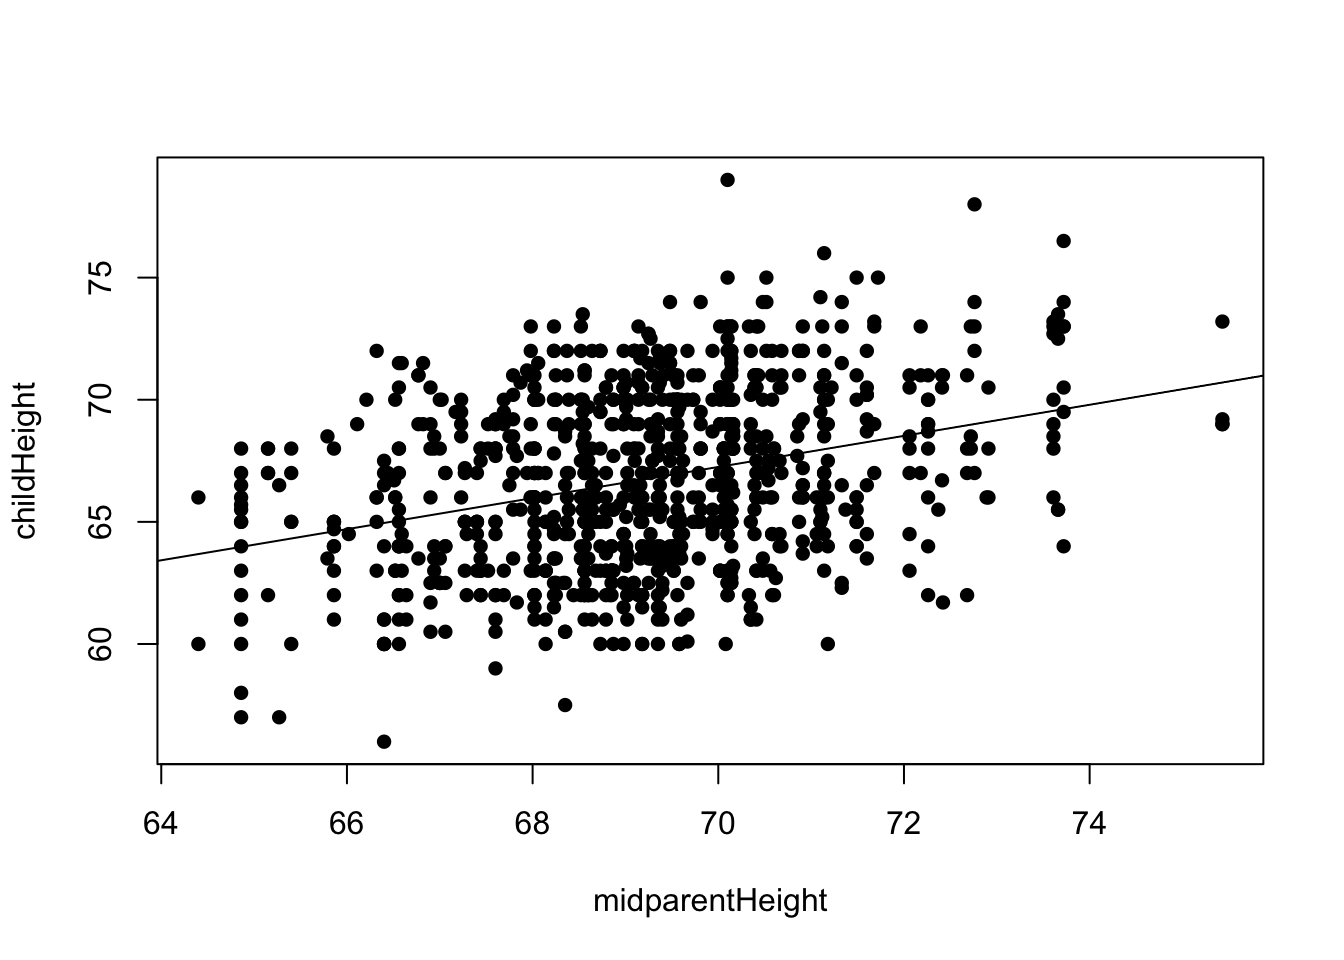
\includegraphics{applied_lecture_notes_files/figure-latex/unnamed-chunk-1-1.pdf}

\begin{verbatim}
##     (Intercept) midparentHeight 
##      22.6362405       0.6373609
\end{verbatim}

Now using Darwin's theory that a parent a sd taller than the mean is
likely to have a child with same characteristics.

\begin{Shaded}
\begin{Highlighting}[]
\NormalTok{(beta1 }\OtherTok{\textless{}{-}}\FunctionTok{with}\NormalTok{(GaltonFamilies, }\FunctionTok{sd}\NormalTok{(childHeight }\SpecialCharTok{/} \FunctionTok{sd}\NormalTok{(midparentHeight))))}
\end{Highlighting}
\end{Shaded}

\begin{verbatim}
## [1] 1.985858
\end{verbatim}

\begin{Shaded}
\begin{Highlighting}[]
\NormalTok{(alpha1 }\OtherTok{\textless{}{-}}\FunctionTok{with}\NormalTok{(GaltonFamilies, }\FunctionTok{mean}\NormalTok{(childHeight)}\SpecialCharTok{{-}}\NormalTok{beta1}\SpecialCharTok{*}\FunctionTok{mean}\NormalTok{(midparentHeight)))}
\end{Highlighting}
\end{Shaded}

\begin{verbatim}
## [1] -70.68889
\end{verbatim}

We see that the black line from Galton's theory is regression to
mediocrity whilst the Darwin theory shows inflated extremal values.

(Regression line in dotted lines, \(y=\alpha_1+\beta_1 x\) in full
line.)

\begin{Shaded}
\begin{Highlighting}[]
\FunctionTok{plot}\NormalTok{(childHeight }\SpecialCharTok{\textasciitilde{}}\NormalTok{ midparentHeight, GaltonFamilies, }\AttributeTok{pch=}\DecValTok{16}\NormalTok{, }\AttributeTok{main=}\StringTok{\textquotesingle{}Children height vs mid{-}parent height\textquotesingle{}}\NormalTok{, }\AttributeTok{xlab=}\StringTok{\textquotesingle{}mid{-}parent height\textquotesingle{}}\NormalTok{, }\AttributeTok{ylab=}\StringTok{\textquotesingle{}children height\textquotesingle{}}\NormalTok{)}
\FunctionTok{abline}\NormalTok{(}\AttributeTok{a=}\NormalTok{alpha1, }\AttributeTok{b=}\NormalTok{beta1)}
\FunctionTok{abline}\NormalTok{(}\FunctionTok{coef}\NormalTok{(lmod), }\AttributeTok{lty=}\DecValTok{5}\NormalTok{)}
\end{Highlighting}
\end{Shaded}

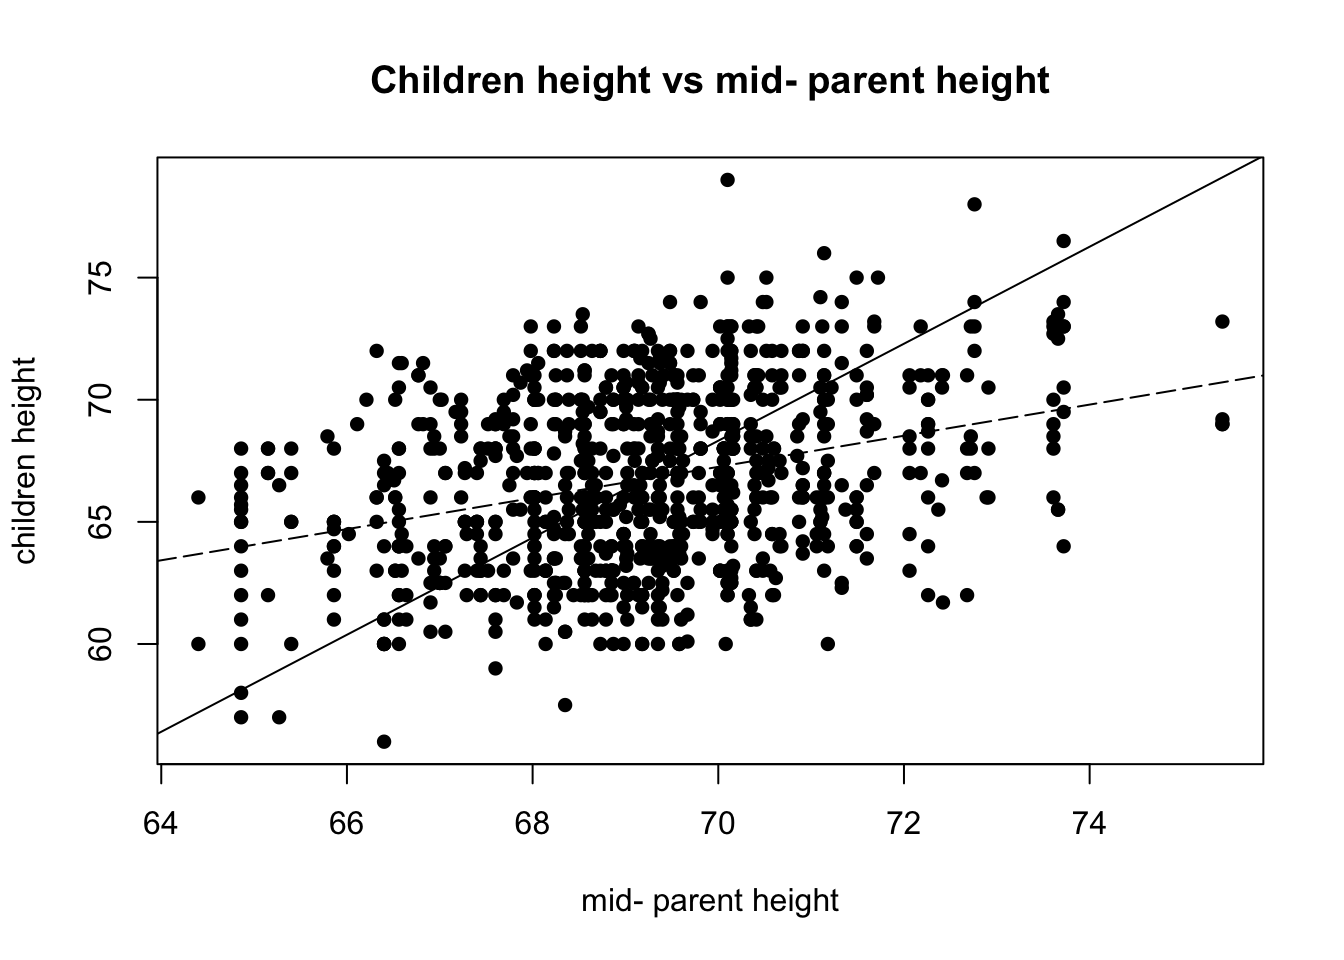
\includegraphics{applied_lecture_notes_files/figure-latex/unnamed-chunk-3-1.pdf}
Why is there regression to mediocrity? Because there's only a smaller
portion of people being a SD taller than the mean (assuming for ex a
normal distribution), so there's a dilution because of the mean. Note
that this doesn't mean that variation across the whole population
diminishes because there's enough random fluctuations across all heights
so that even though we say an individual is 1 standard deviation above
average implies that his child can expect a less than 1 standard
deviation above average, the total variability is kept.

\hypertarget{lecture-2-linear-regression}{%
\section{Lecture 2: linear
regression}\label{lecture-2-linear-regression}}

\hypertarget{regression-response-covariates}{%
\subsection{Regression: response,
covariates}\label{regression-response-covariates}}

\hypertarget{simple-linear-regression}{%
\subsubsection{Simple linear
regression}\label{simple-linear-regression}}

\[\forall i=1,\dots, n:\ \ \ y_i=\alpha+\beta x_i+\varepsilon_i\] We
can't fit a straight line to our data points with it going through all
the points, Galton introduces the idiosyncratic error through residuals
captured with \(\varepsilon\).

\hypertarget{least-square-estimate}{%
\subsubsection{Least square estimate}\label{least-square-estimate}}

Measure ``closeness'' through SSE (sum of squared errors):
\[SSE=\sum_i [y_i-(\alpha+\beta x_i)]^2\]

Least squares estimate:
\[(\hat{\alpha},\hat{\beta})=\arg\min_{a, b}\sum_i [y_i-(\alpha+\beta x_i)]^2=SSE(a,b)\]
Ofc we can look at first order conditions. Alternatively, an intuition
on fitting least squares is noting that
\[\min SSE(a,b)=\sum_i [y_i-(\alpha+\beta x_i)]^2=\sum_i [y_i-\bar{y}-(\alpha+\beta (x_i-\bar{x})]^2\]
We can set our intercept to 0 going through middle points. Then let the
slope be
\(\hat{\beta}=\frac{\sum_i (y_i-\bar{y})(x_i-\bar{x})}{\sum_i (x_i-\bar{x})^2}\)
and intercept \(\hat{\alpha}=\bar{y}-\hat{\beta}\bar{x}\).

Can rewrite
\(\hat{\beta}=\frac{Cov(x,y)}{Var(x)}=\rho_{x,y}\frac{s_y}{s_x}\) We can
recognise that regression to the mean (mediocrity) if \(\rho_{x,y}<1\).

Fitted values: \(\hat{y}_i=\hat{\alpha}+\hat{\beta}x_i\)

Fitted line: \((\hat{y}_i-\bar{y})=\hat{\beta}(x_i-\bar{x})\)

\hypertarget{residuals-properties}{%
\subsubsection{Residuals' properties}\label{residuals-properties}}

-SSE is minimised.\newline -orthogonality properties :\newline 
1. \(\sum_i\hat{\varepsilon}_i=0\) ie error is null on average\newline
2. \(\sum_i x_i\hat{\varepsilon}_i=Cov(x,\hat{\varepsilon})=0\) (if it
isn't null, means there's still correlation in \(x\) that we could fit
our data better)\newline
3. \(\sum_i\hat{y}_i\hat{\varepsilon}_i=0\) (as a linear combination of
1. and 2.)

\hypertarget{optimality-of-lse}{%
\subsubsection{Optimality of LSE}\label{optimality-of-lse}}

Two reasons for choosing LSE are relying on its simplicity.

\hypertarget{blue}{%
\paragraph{BLUE}\label{blue}}

The LSE is the BLUE ie Best Linear Unbiased Estimator ie restricting
ourselves to the class of linear estimators, this is the choice with
best properties. Consider \(b=\sum_i a_i(y_i-\bar{y})\). Want to
minimise variance of the estimator assuming we constraint it to be
unbiased.

\(\mathbb{E}_{\varepsilon}(y_i-\bar{y})=\beta (x_i-\bar{x})\)

\textbf{Assumption:} \(Var(\varepsilon_i)=\sigma^2\)\newline

-Bias \(=\beta-\mathbb{E}_{\varepsilon}(b)\)\newline  -Variance
\(=var_\varepsilon(b)=\sum_i (a_i-\bar{a})\)\newline 

Solving the following for BLUE=\(\min_a\sum_i (a_i-\bar{a})^2\) subject
to \(\sum_i a_i(x_i-\bar{x})=1\)\newline  Using Lagrange multiplier,
first order condition writes
\(a_i=\frac{x_i-\bar{x}}{\sum_j (x_j-\bar{x})^2}\)

\hypertarget{interpretation-of-fit}{%
\paragraph{Interpretation of fit}\label{interpretation-of-fit}}

\[\mathbb{E}[Y-(a+bX)]^2=\mathbb{E}[Y-\mathbb{E}(Y|X)]^2+\mathbb{E}[\mathbb{E}(Y|X)-(a+bX)]^2\]

This means LSE allows a linear approximation to \(\mathbb{E}(Y|X)\). The
difference with this and the original linear regression, is that by
taking the conditional expectation, we average out the idiosyncratic
error and approximate over the conditional mean which allows our design
to be random as well.

\hypertarget{examples}{%
\paragraph{Examples}\label{examples}}

-Binary \(X\)\newline  Say \(X\in\{0,1\}\)
\[\mathbb{E}(Y|X=x)=\mu_1\mathbb{1}(x=1)+\mu_0\mathbb{1}(x=0)=(\mu_1-\mu_0)x+\mu_0\]

Control group being 0, treatment group 1. Intercept gives the baseline
effect, slope the treatment effect. If \(X\) is binary, LS always works,
it delivers treatment and baseline effect directly.

-Depends on both \(\mathbb{E}(Y|X)\) and the distribution of \(X\) as
well ! Read Buja et al.~2019, Statistical Science on
\url{https://arxiv.org/pdf/1404.1578.pdf}. Often times a linear model is
not sufficient if we're not looking at local \(x\).

-Stein's Identity Assumption: \textbf{Assume} \(X\) is Gaussian.
\emph{Theorem}: If \(X\sim N(0,1)\), then
\(\mathbb{E}(Xg(X))=\mathbb{E}g'(X)\).

Estimand of the slope: set \(f(X)=\mathbb{E}(Y|X)\), we get
\(\mathbb{E}(Y-(a+bX))^2\to\beta=\mathbb{E}(f'(X))\)

\hypertarget{summary}{%
\subsubsection{Summary}\label{summary}}

For OLS estimate we have -explicit form:
\(\hat{\beta}=\frac{Cov(x,y)}{Var(x)}=\rho_{x,y}\frac{s_y}{s_x}\)

-for residuals, they are uncorrelated with fitted value, covariate:
\(\sum_i x_i\hat{\varepsilon}_i=Cov(x,\hat{\varepsilon})=0\)

-interpretation:

\begin{verbatim}
-treatment effect
  
-linear approximation to conditional mean
  
-slope: (Stein's theorem) averaged derivative under Gaussian
\end{verbatim}

\hypertarget{lecture-3-inference}{%
\section{Lecture 3: Inference}\label{lecture-3-inference}}

\hypertarget{scope-of-statistical-inference}{%
\subsection{Scope of statistical
inference}\label{scope-of-statistical-inference}}

Inference needs assumptions.

-Point estimation \(\hat{\theta}(X)\)

-Confidence interval
\(P(\hat{\theta}_L(X)\leq\theta\leq\hat{\theta}_U(X))\geq 1-\alpha\)

-Hypothesis testing : reject \(H_0\) if \(X\in\mathcal{R}\),
\(H_0 :\theta=\theta_0\)

-Testing
\(\mathcal{R}^c=\{X:\hat{\theta}_L(X)\leq\theta_0\leq\hat{\theta}_U(X)\}\)
(dual of confidence interval)

-Asymmetry: can reject but cannot \emph{confirm}

\hypertarget{inference-for-slr}{%
\subsection{Inference for SLR}\label{inference-for-slr}}

\hypertarget{interpretation}{%
\subsubsection{Interpretation}\label{interpretation}}

\emph{Assuming} -Linearity \(E(Y|X)=\alpha+\beta X\)

-Homoscedasticity \(Var(\varepsilon_i)=\sigma_0^2\)

-Independence of errors \(\varepsilon_i\perp\varepsilon_j\)

-Normality of errors \(\varepsilon_i\sim N(0,\sigma_0^2)\)

\begin{Shaded}
\begin{Highlighting}[]
\FunctionTok{summary}\NormalTok{(lmod)}
\end{Highlighting}
\end{Shaded}

\begin{verbatim}
## 
## Call:
## lm(formula = childHeight ~ midparentHeight, data = GaltonFamilies)
## 
## Residuals:
##     Min      1Q  Median      3Q     Max 
## -8.9570 -2.6989 -0.2155  2.7961 11.6848 
## 
## Coefficients:
##                 Estimate Std. Error t value Pr(>|t|)    
## (Intercept)     22.63624    4.26511   5.307 1.39e-07 ***
## midparentHeight  0.63736    0.06161  10.345  < 2e-16 ***
## ---
## Signif. codes:  0 '***' 0.001 '**' 0.01 '*' 0.05 '.' 0.1 ' ' 1
## 
## Residual standard error: 3.392 on 932 degrees of freedom
## Multiple R-squared:  0.103,  Adjusted R-squared:  0.102 
## F-statistic:   107 on 1 and 932 DF,  p-value: < 2.2e-16
\end{verbatim}

\emph{Quantities to interpret out of output}

-regression coefficients \(\alpha\), \(\beta\) as

\begin{verbatim}
-point estimates:
\end{verbatim}

\(\hat{\alpha}=\bar{y}-\hat{\beta}\bar{x}\) and
\$\hat{\beta}=\frac{\sum_i (x_i-\bar{x})(y_i-\bar{y})}{\sum_i (x_i-\bar{x})$2}

\begin{verbatim}
-sampling distribution 
\end{verbatim}

\(\hat{\beta}\sim N(\beta,\frac{\sigma_0^2}{[\sum_i (x_i-\bar{x})^2]^{-1}})\),
\(\bar{y}\perp\hat{\beta}\bar{x}\)

-error variance \(\sigma_0^2\)

\begin{verbatim}
-error variance from residuals 
\end{verbatim}

\(r_i=y_i-\hat{y}_i\) to \(\hat{\sigma}^2=\frac{1}{n-2}\sum_i r_i^2\)

\begin{verbatim}
-residual variance 
\end{verbatim}

\(\hat{\sigma}^2\sim\sigma_0^2\chi_{n-2}^2/(n-2)\) note that
\((\hat{\alpha},\hat{\beta})\perp\hat{\sigma}^2\)

-prediction: \(y_{new}=\alpha+\beta x_{new}+\varepsilon_{new}\)

\hypertarget{test-of-significance}{%
\subsubsection{Test of significance}\label{test-of-significance}}

Under \(H_0 :\beta=0\),
\(\frac{\hat{\beta}}{\hat{\sigma}[\sum_i (x_i-\bar{x})^2]^{-1/2}}\sim t_{n-2}\)
Under \(H_0 :\alpha=0\),
\(\frac{\hat{\alpha}}{\hat{\sigma}[\frac{1}{n}+\frac{\bar{x}^2}{\sum_i (x_i-\bar{x})^2}]^{1/2}}\sim t_{n-2}\)

Remark: many problems with t-value, needs \emph{normality} and
\emph{independence}. However, even when assumptions don't hold, can
somehow make it work.

\hypertarget{anova-and-r2}{%
\subsection{ANOVA and R2}\label{anova-and-r2}}

\hypertarget{anova}{%
\subsubsection{ANOVA}\label{anova}}

Decomposition of variation: recall in Galton's example, we see variance
introduced by parent's height and intrinsic variance.

\begin{figure}
\centering
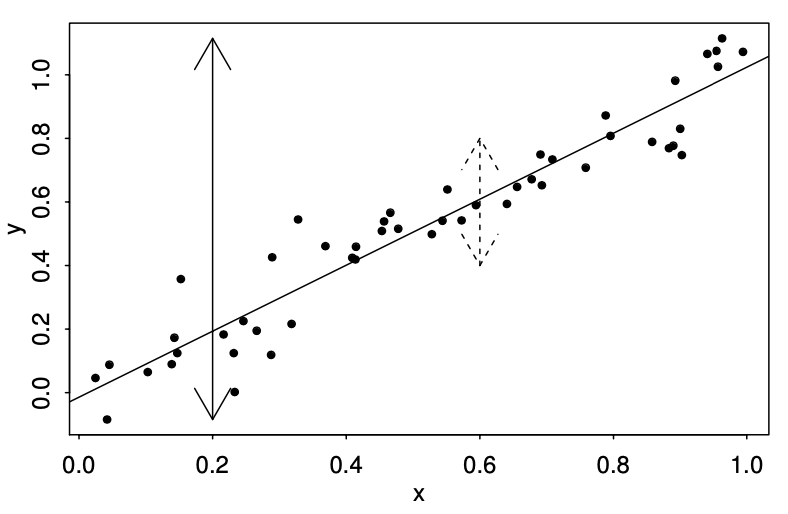
\includegraphics{/Users/h2jw/Documents/GitHub/STATGRXXXX/STATGR6101/images/galton.png}
\caption{When \(x\) is not known, the best predictor of \(y\) is
\(\bar{y}\) and the variation is denoted by the dotted line. When \(x\)
is known, we can predict \(y\) more accurately by the solid line.
\(R^2\) is related to the ratio of these two variances.}
\end{figure}

We use analysis of variance:
\[\underbrace{\sum_i(y_i-\bar{y})^2}_{SST}=\underbrace{\sum_i(y_i-\hat{y})^2}_{SSE}+\underbrace{\sum_i(\hat{y}_i-\bar{y})^2}_{SSR}\]

-\(SST\): total variation

-\(SSE\): unexplained variation

-\(SSR\): variation explained by regression

\hypertarget{goodness-of-fit}{%
\subsubsection{Goodness of fit}\label{goodness-of-fit}}

Or \(R^2\) the coefficient of determination to assess prediction power.
\[R^2=1-\frac{\sum_i (y_i-\hat{y_i})^2}{\sum_i (y_i-\bar{y})^2}=\frac{SSR}{SST}\]
Note that for SLR, \(R^2=\rho_{X,Y}^2\).

\(R^2\) gives an idea of how much information our predictors give to our
response: goodness of fit. However, there is no ``threshold'' value for
a good \(R^2\).

\begin{figure}
\centering
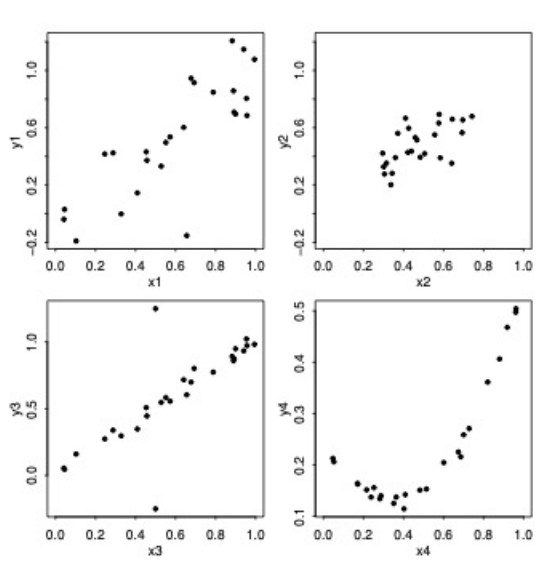
\includegraphics{/Users/h2jw/Documents/GitHub/STATGRXXXX/STATGR6101/images/R2_comp.png}
\caption{Four simulated datasets where \(R^2\) is about 0.65. The plot
on the upper left is well-behaved for \(R^2\). In the plot on the upper
right, the residual variation is smaller than the first plot but the
variation in \(x\) is also smaller so \(R^2\) is about the same. In the
plot on the lower left, the fit looks strong except for a couple of
outliers while on the lower right, the relationship is quadratic.}
\end{figure}

We can also rewrite F-test in terms of \(SSE\), \(SSR\): note that
\(SSE\sim\sigma^2\chi_{n-2}^2\), \(SSR\sim\sigma^2\chi_1^2\) with
\(SSE\perp SSR\). Then the F-test for \(H_0 :\beta=0\) :
\[F=\frac{SSR}{SSE/(n-2)}\sim F_{1,n-2}\]

\hypertarget{lecture-4-prediction}{%
\section{Lecture 4: Prediction}\label{lecture-4-prediction}}

\emph{Recap} How to make sense of \(R\) output: -Parameter estimation

-ANOVA analysis of variance: \(SST=SSE+SSR\)

-Inference under assumptions:

-linearity

-homoscedasticity

-independence of errors

-normality of errors

\hypertarget{scope-of-prediction}{%
\subsection{Scope of prediction}\label{scope-of-prediction}}

We observe a new set of observation not used to estimate
\(\hat{\beta}\): \(y_{new}=\alpha+x_{new}\cdot\beta+\epsilon_{new}\).

-Estimate: \(\hat{y}_{new}=\hat{\alpha}+x_{new}\cdot\hat{\beta}\)

-Confidence interval: to calculate CI, we need to compute the variance
of our estimator
\[Var(\hat{y}_{new}|x, x_{new})=Var(\hat{\alpha}+ x_{new}\cdot\hat{\beta}|x,x_{new})\\
=\sigma^2\big(\frac{1}{n}+\frac{(x_{new}-\bar{x})^2}{\sum_j (x_j-\bar{x})^2}\big)\]

-Sampling distribution:
\(\hat{y}_{new}\sim N\big(\alpha+x_{new}\cdot\beta,\sigma^2\big(\frac{1}{n}+\frac{(x_{new}-\bar{x})^2}{\sum_j (x_j-\bar{x})^2}\big)\big)\)
and can infer the \emph{CI} for mean of \(y_{new}\):
\$C\_q=\big[\hat{\alpha}+ x_{new}\cdot\hat{\beta}\pm t_{n-2, 1-q/2}\cdot\sqrt{\sigma^2\big(\frac{1}{n}+\frac{(x_{new}-\bar{x})^2}{\sum_j (x_j-\bar{x})^2}\big)}\big] \$

-Prediction interval: we're typically interested in an interval for the
actual observation \(y_{new}\) rather than the mean of \(y_{new}\). To
calculate the variance of the prediction, see that:
\[Var(y_{new}-\hat{y}_{new}|x, x_{new})=Var(y|x, x_{new})-Var(\hat{y}_{new}|x, x_{new})\\
=\sigma^2\big[ 1+\frac{1}{n}+\frac{(\bar{x}-x_{new})^2}{\sum_j (x_j-\bar{x})^2}\big]\]
which yields \emph{prediction interval}:
\(P_q=\big[\hat{\alpha}+ x_{new}\cdot\hat{\beta}\pm t_{n-2, 1-q/2}\cdot\sqrt{\sigma^2\big(1+\frac{1}{n}+\frac{(x_{new}-\bar{x})^2}{\sum_j (x_j-\bar{x})^2}\big)}\big]\)

\begin{Shaded}
\begin{Highlighting}[]
\NormalTok{newdata }\OtherTok{\textless{}{-}}\FunctionTok{data.frame}\NormalTok{(}\AttributeTok{midparentHeight=}\DecValTok{70}\NormalTok{)}
\FunctionTok{predict}\NormalTok{(lmod, newdata, }\AttributeTok{interval=}\StringTok{\textquotesingle{}none\textquotesingle{}}\NormalTok{)}
\end{Highlighting}
\end{Shaded}

\begin{verbatim}
##       1 
## 67.2515
\end{verbatim}

\begin{Shaded}
\begin{Highlighting}[]
\FunctionTok{predict}\NormalTok{(lmod, newdata, }\AttributeTok{interval=}\StringTok{\textquotesingle{}confidence\textquotesingle{}}\NormalTok{)}
\end{Highlighting}
\end{Shaded}

\begin{verbatim}
##       fit      lwr      upr
## 1 67.2515 67.01352 67.48948
\end{verbatim}

\begin{Shaded}
\begin{Highlighting}[]
\FunctionTok{predict}\NormalTok{(lmod, newdata, }\AttributeTok{interval=}\StringTok{\textquotesingle{}predict\textquotesingle{}}\NormalTok{)}
\end{Highlighting}
\end{Shaded}

\begin{verbatim}
##       fit      lwr      upr
## 1 67.2515 60.59097 73.91204
\end{verbatim}

\hypertarget{assumptions}{%
\subsection{Assumptions}\label{assumptions}}

We check our assumptions on the residuals using the diagnostic plots.
Residuals vs fitted to check for I-IV (linearity, homoscedasticity, no
collinearity, independent errors) and Q-Q to check for V (normality of
errors).

\begin{Shaded}
\begin{Highlighting}[]
\FunctionTok{par}\NormalTok{(}\AttributeTok{mfrow=}\FunctionTok{c}\NormalTok{(}\DecValTok{1}\NormalTok{,}\DecValTok{2}\NormalTok{))}
\FunctionTok{plot}\NormalTok{(lmod, }\AttributeTok{which=}\DecValTok{1}\NormalTok{, }\AttributeTok{pch=}\DecValTok{19}\NormalTok{)}
\FunctionTok{plot}\NormalTok{(lmod, }\AttributeTok{which=}\DecValTok{2}\NormalTok{)}
\end{Highlighting}
\end{Shaded}

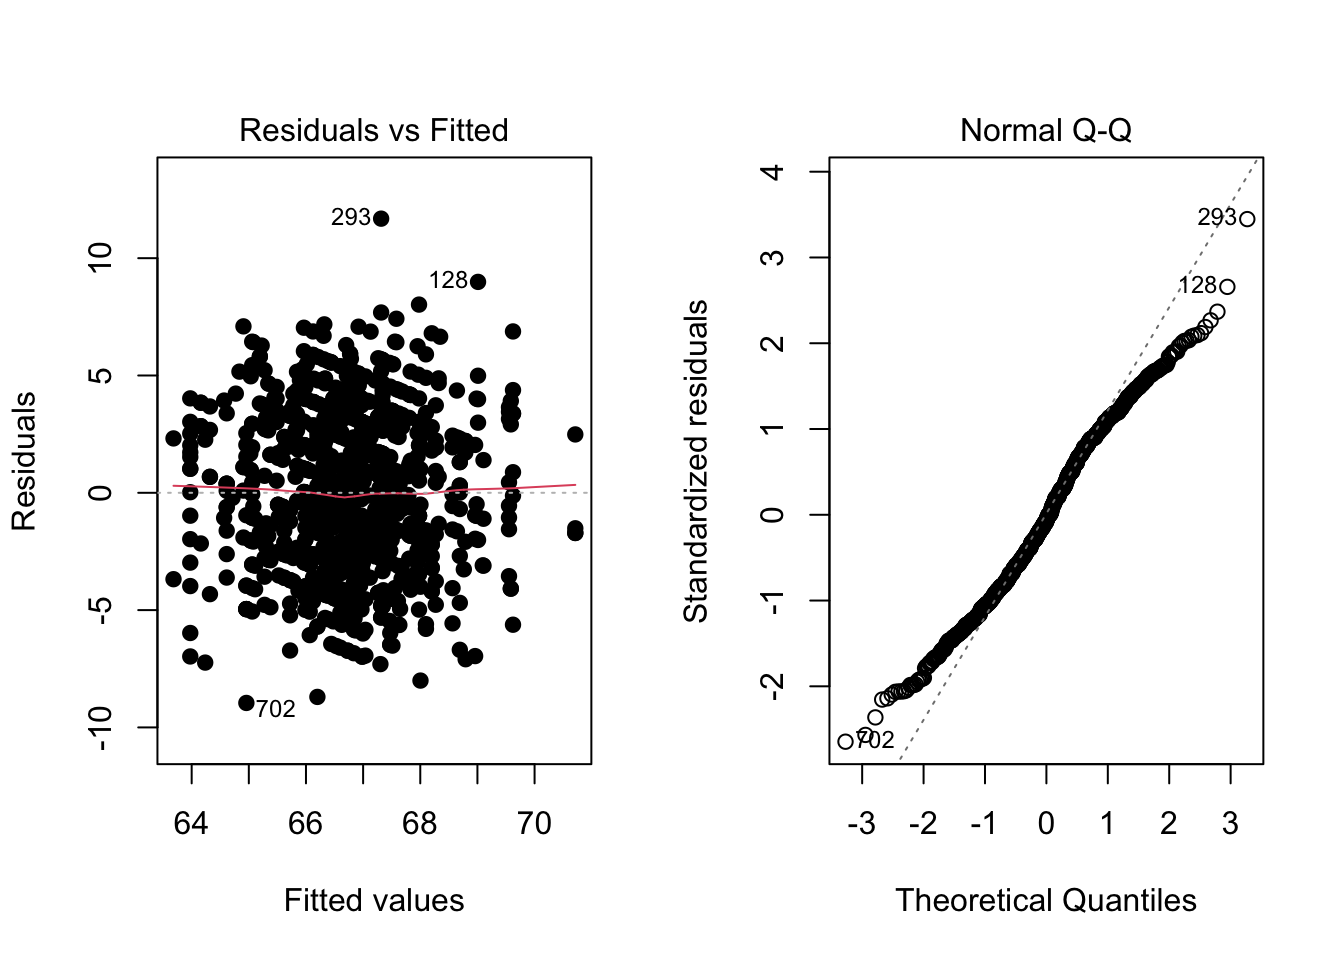
\includegraphics{applied_lecture_notes_files/figure-latex/unnamed-chunk-6-1.pdf}

\hypertarget{if-normality-doesnt-hold}{%
\subsubsection{If normality doesn't
hold}\label{if-normality-doesnt-hold}}

What happens when we have deviation from normal?

The normality assumption (V) can be dropped if sample size is big
enough. For this, we use the Central limit theorem and Slutsky theorem.

CLT:
-\(\hat{\beta}\to_d N\big(\beta,\sigma_0^2\big[\sum_i (x_i-\bar{x})^2\big]^{-1}\big)\)

-\(\hat{\alpha}\to_d N\big(\alpha,\sigma_0^2\big[\frac{1}{n}+\frac{\bar{x}^2}{\sum_i (x_i-\bar{x})^2}\big]\big)\)

Note that those distribution depend on \(\sigma_0^2\). We use Slutsky's
theorem so that inference is valid in those expressions. Let
\(\hat{\sigma}^2\to_P\sigma_0^2\), then

-under \(H_0 :\beta=0\),
\(\frac{\hat{\beta}}{\hat{\sigma}[\sum_i (x_i-\bar{x})^2]^{-1/2}}\to_d N(0,1)\)

-under \(H_0 :\alpha=0\),
\(\frac{\hat{\alpha}}{\hat{\sigma}[\frac{1}{n}+\frac{\bar{x}^2}{\sum_i (x_i-\bar{x})^2}]^{-1/2}}\to_d N(0,1)\)

-For large \(n\), \(t_{n-2}\to_d N(0,1)\).

Which justifies that normality can be dropped if the sample size is
large enough.

\hypertarget{if-heteroscedascity}{%
\subsubsection{If heteroscedascity?}\label{if-heteroscedascity}}

Assume now that \(Var(\epsilon_i)=\sigma_i^2\). We are outside the
framework of homoscedastic errors.

-If \(\sigma_i\) are known, we can use the sandwich formula:
\(Var(\hat{\beta})=\frac{\sum_i\sigma_i^2 (x_i-\bar{x})^2}{[\sum_i (x_i-\bar{x})^2]^2}\)

-However, we can not usually estimate \(\sigma_i^2\). But by WLLN with
the residuals \(r_i\), the following holds true:
\[\widehat{Var{\hat{\beta}}}:=\frac{\sum_i r_i^2 (x_i-\bar{x})^2}{[\sum_j (x_j-\bar{x})^2]^2}\to_P Var(\hat{\beta})\]
So we can give some slack to the homoscedascity assumption without
loosing inference. The point estimate is still gonna be valid,
\emph{however} this needs for standard error and inferences to be
adjusted.

\hypertarget{lecture-5-inference-in-linear-models}{%
\section{Lecture 5: Inference in linear
models}\label{lecture-5-inference-in-linear-models}}

\hypertarget{assumptions-in-lm}{%
\subsection{Assumptions in LM}\label{assumptions-in-lm}}

\emph{Recap} Assumption for inference : Check residuals plots

-Normality: \(\varepsilon_i\sim\mathcal{N}(0,1)\)

-Homoscedasticity: \(Var(\varepsilon_i)=\sigma_0^2\) under mild
conditions (large sample size), can get a valid estimator even without
homoscedasticity using SSR

-Independence of errors

-Linearity

\hypertarget{inference-when-non-linearity}{%
\subsubsection{Inference when non
linearity?}\label{inference-when-non-linearity}}

Non linearity: assume model \(E(Y|X)=\alpha+\beta X+\delta(X)\) where
\(\delta(X)\) models the non linearity. By assumption of LS,
\(E(\delta(X))=E(X\delta(X))=0\). Interpretation of our estimator
changes slightly, however still possible in terms of variation of
quantities with care. Inference is affected however, Let
\(Y_i=\alpha+\beta X_i+\delta(X_i)+\varepsilon_i\) and set
\(\hat{\varepsilon}_i=\delta(X_i)+\varepsilon_i\). Therefore: Then
\(\hat{\beta}\underset{d}{\rightarrow}N(\beta,\frac{\delta_{\hat{\varepsilon}}^2}{\sum_i (x_i-\bar{x})^2})\)
Noting \(\sigma^2=\sigma_0 ^2+E(\delta(X)^2)\) yields
\(\hat{\beta}\underset{d}{\rightarrow}N(\beta,\frac{\sigma^2}{\sum_i (x_i-\bar{x})^2})\)

Slight caveat, we assume here that \(\sigma_0 ^2+E(\delta(X)^2)\) means
\(\delta(X_i)+\varepsilon_i\) are uncorrelated. Moreover, we need to be
careful of fixed or random design. If random design, no issue with
heteroscedasticity since it averages out. If fixed design, we need to
also take care of heteroscedasticity.

\hypertarget{what-if-our-errors-arent-independent}{%
\subsubsection{What if our errors aren't
independent?}\label{what-if-our-errors-arent-independent}}

Independence: \(Cov(\varepsilon_i,\varepsilon_j)=0\).

However, if residuals not uncorrelated, we have
\(Cov(\varepsilon_i,\varepsilon_j)=\sigma_{ij}\) then
\(Var(\hat{\beta})=\frac{\sum_{i,j}\sigma_{ij}(x_i-\bar{x})(x_j-\bar{x})}{(\sum_i (x_i-\bar{x})^2)^2}\)

Central limit theorem only holds under \emph{weak dependence} !
Independence is a very strong assumption, weakening it is possible
however it's not possible to get rid of it contrary to
heteroscedasticity for example. Usually, we do not get around it, but
try to model the dependence or only keep the point estimate.

Implications: -point estimate is still valid

-standard error estimate is \emph{invalid}

-\emph{interpretation} different !

\hypertarget{scatterplot-and-modelling}{%
\subsection{Scatterplot and modelling}\label{scatterplot-and-modelling}}

Data analysis: overview of the data Scatterplots relevant when not too
many variables.

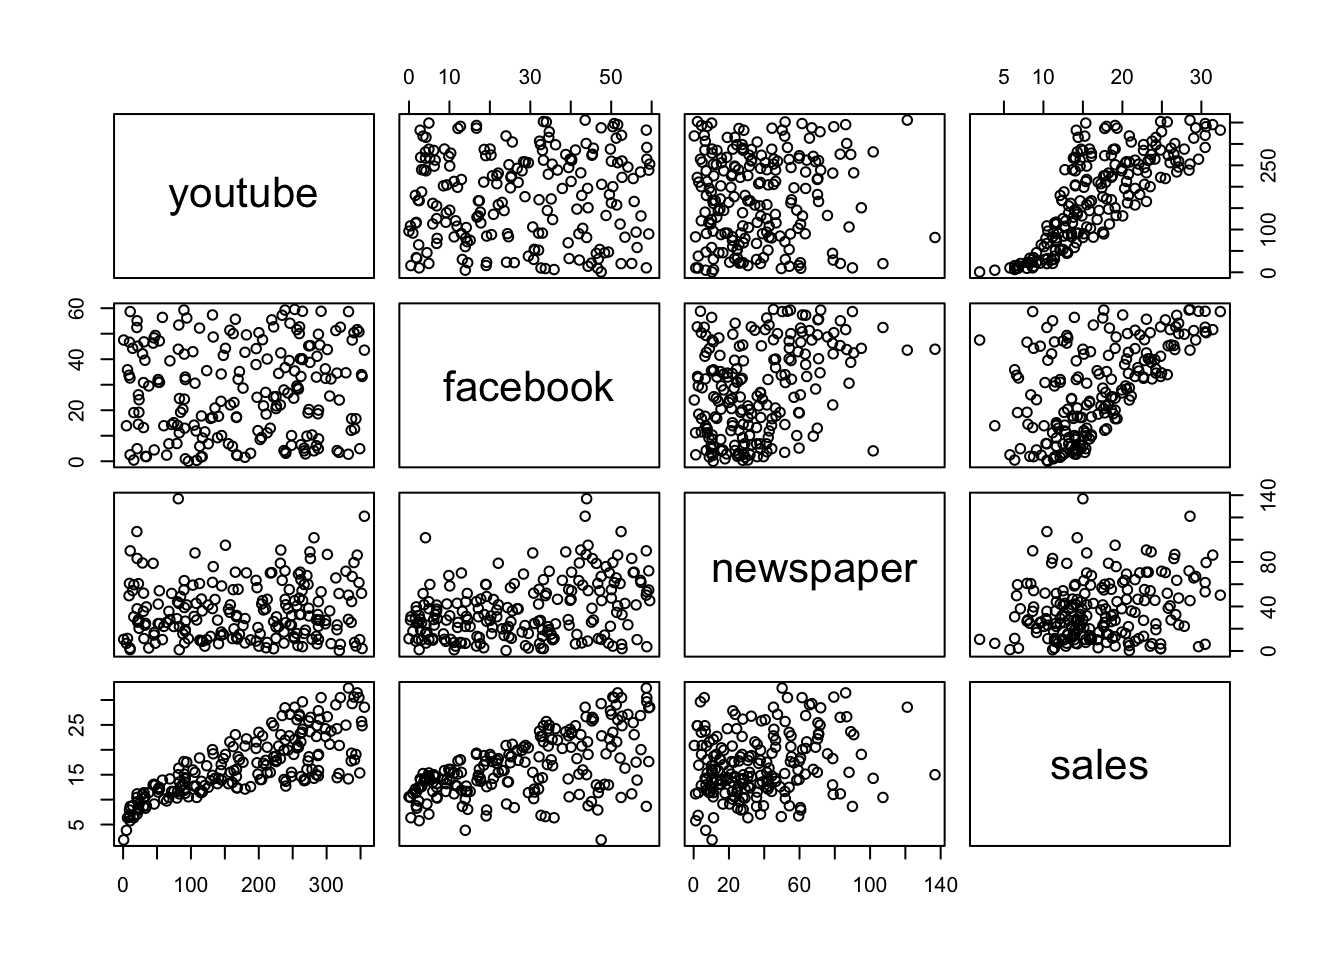
\includegraphics{applied_lecture_notes_files/figure-latex/unnamed-chunk-7-1.pdf}

\hypertarget{multiple-linear-regression}{%
\subsubsection{Multiple linear
regression}\label{multiple-linear-regression}}

\begin{Shaded}
\begin{Highlighting}[]
\NormalTok{res.lm }\OtherTok{\textless{}{-}}\FunctionTok{lm}\NormalTok{(sales }\SpecialCharTok{\textasciitilde{}}\NormalTok{ youtube}\SpecialCharTok{+}\NormalTok{facebook}\SpecialCharTok{+}\NormalTok{newspaper, }\AttributeTok{data=}\NormalTok{marketing) }
\FunctionTok{summary}\NormalTok{(res.lm)}
\end{Highlighting}
\end{Shaded}

\begin{verbatim}
## 
## Call:
## lm(formula = sales ~ youtube + facebook + newspaper, data = marketing)
## 
## Residuals:
##      Min       1Q   Median       3Q      Max 
## -10.5932  -1.0690   0.2902   1.4272   3.3951 
## 
## Coefficients:
##              Estimate Std. Error t value Pr(>|t|)    
## (Intercept)  3.526667   0.374290   9.422   <2e-16 ***
## youtube      0.045765   0.001395  32.809   <2e-16 ***
## facebook     0.188530   0.008611  21.893   <2e-16 ***
## newspaper   -0.001037   0.005871  -0.177     0.86    
## ---
## Signif. codes:  0 '***' 0.001 '**' 0.01 '*' 0.05 '.' 0.1 ' ' 1
## 
## Residual standard error: 2.023 on 196 degrees of freedom
## Multiple R-squared:  0.8972, Adjusted R-squared:  0.8956 
## F-statistic: 570.3 on 3 and 196 DF,  p-value: < 2.2e-16
\end{verbatim}

Equivalent to list all variables or to use .

\begin{Shaded}
\begin{Highlighting}[]
\NormalTok{res.lm }\OtherTok{\textless{}{-}}\FunctionTok{lm}\NormalTok{(sales }\SpecialCharTok{\textasciitilde{}}\NormalTok{ ., }\AttributeTok{data=}\NormalTok{marketing) }
\FunctionTok{summary}\NormalTok{(res.lm)}
\end{Highlighting}
\end{Shaded}

\begin{verbatim}
## 
## Call:
## lm(formula = sales ~ ., data = marketing)
## 
## Residuals:
##      Min       1Q   Median       3Q      Max 
## -10.5932  -1.0690   0.2902   1.4272   3.3951 
## 
## Coefficients:
##              Estimate Std. Error t value Pr(>|t|)    
## (Intercept)  3.526667   0.374290   9.422   <2e-16 ***
## youtube      0.045765   0.001395  32.809   <2e-16 ***
## facebook     0.188530   0.008611  21.893   <2e-16 ***
## newspaper   -0.001037   0.005871  -0.177     0.86    
## ---
## Signif. codes:  0 '***' 0.001 '**' 0.01 '*' 0.05 '.' 0.1 ' ' 1
## 
## Residual standard error: 2.023 on 196 degrees of freedom
## Multiple R-squared:  0.8972, Adjusted R-squared:  0.8956 
## F-statistic: 570.3 on 3 and 196 DF,  p-value: < 2.2e-16
\end{verbatim}

MLR is a generalisation of SLR.

\[y_i=\alpha+\beta_1 x_{i1}+\beta_2 x_{i2}+\dots+\beta_p x_{ip}+\varepsilon_i\]

Idea with MLR is to observe variations of our variable with a change of
each covariate, when \emph{all others are fixed}.

Back to SLR : \(Y=\alpha+\beta X+\varepsilon\), interpretation with
confounders so writing \(Y=Z+\varepsilon'\). This can be rewritten as
\(X=YZ+\varepsilon''\) where \(Z\) is the matrix of confounders. And the
interest of the regression depends on our identification of confounders.
This is the backing behind the idea of identifying change with ``other
covariates fixed''. MLR is a \(p\)-component estimation problem of
\(\beta\) (we can get rid of \(\alpha\) by substracting the mean). Note
that \(y_i=x_i^T\beta+\varepsilon_i\) in MLR.

Our model rewrites to : \[Y=X\beta+\varepsilon\]

with
\(Y=(y_1,\dots, y_n)^T,\varepsilon=(\varepsilon_1,\dots,\varepsilon_n)^T\in\mathbb{R}^n, X=(x_1,\dots, x_n)\in\mathbb{R}^{n\times p}\)
where \(x_i=(x_{i1},\dots, x_{ip})^T\in\mathbb{R}^p\) and
\(\beta=(\beta_1,\dots,\beta_p)^T\in\mathbb{R}^p\)

\hypertarget{least-squares-in-mlr}{%
\subsubsection{Least squares in MLR}\label{least-squares-in-mlr}}

notation: \(||a||^2=\sum_i a_i^2\)

To estimate the LS solution, use the MLE for independent normal errors,
then:

\[\hat{\beta}\in\arg\min_{b\in\mathbb{R}^p}||Y-Xb||^{2}\]

We fit a p-hyperplane through our data in an n-dimensional space. We
might have no solutions, \ldots, even infinite number of solutions.

A useful trick is to rewrite the following:

\begin{eqnarray*}
||Y-Xb||^2 &=& (Y-Xb)^T(Y-Xb)\\
&=& (Y^T+b^T X^T)(Y-Xb)\\
&=& Y^T Y+b^T X^T X b-2 Y^T X b  
\end{eqnarray*}

Gradient of SS : \(\nabla_b ||Y-Xb||^2=2(X^T X b-X^T Y)= 0\)

Which yields if \(X\) is full rank, finally
\(\hat{\beta}=(X^{T}X)^{-1}(X^{T}Y)\).

\hypertarget{geometrical-interpretation}{%
\subsection{Geometrical
interpretation}\label{geometrical-interpretation}}

We want to picture our covariate space as the column space of \(X\).
\[\mathcal{C}(X)=\{\theta:\theta=Xb, b\in\mathbb{R}^p\}\\
\hat{\theta}=\arg\min_\theta\{||\theta-Xb ||^2 : b\in\mathbb{R}^p\}\]

The linear model is the space spanned by the \(p\)-columns of X. The
question we're asking ourselves while fitting our linear model is:
What's the closest point to \(Y\) on the linear space spanned by \(X\) ?
This means that fitting a lm is basically obtaining a projection of
\(Y\) on the spanned column space of \(X\).

Note: projection properties of \(E(Y|X)=X\beta\).

Check-out Bill Benter (how he refined a statistical model to perfect his
gambling).

\emph{Summary of 4,5}

\begin{tabular}{|c| c c c c |}
\hline 
 & non linearity & heteroscedasticity & non independence of errors & non normality of errors\\\hline 
point estimates &\color{red}{not valid}&\color{green}{valid}&\color{green}{valid}&\color{green}{valid}\\
standard errors &\color{red}{not valid}&\color{green}{valid}if adjusted with Sandwich formula &\color{red}{not valid}&\color{green}{valid}\\
interpretation &\color{green}{valid}with care that there is non linearity &\color{green}{valid}if adjusted with Sandwich &\color{green}{valid}under weak independence (CLT holds) &\color{green}{valid}\\
significance &\color{red}{not valid}&\color{green}{valid}&\color{red}{not valid}&\color{green}{valid}only for large sample size\\\hline 
\end{tabular}

\hypertarget{lecture-6-diagnostics}{%
\section{Lecture 6: Diagnostics}\label{lecture-6-diagnostics}}

\emph{Recap} Regression as a projection : \(P_X :=X(X^T X)^{-1}X^T\) the
projection matrix or \emph{hat matrix}. See that \(P_X X=X\) and
\(P_Y=P_X Y=X(X^T X)^{-1}X^T Y=X\hat{\beta}=\hat{\theta}=\hat{Y}\) gives
you the fitted values \(\hat{Y}\).

Notice the dimensions of the projection matrix:
\(P_X=\underbrace{\underbrace{X}_{n\times p}\underbrace{(X^T X)^{-1}}_{p\times p}\underbrace{X^T}_{p\times n}}_{n\times n}\).

\hypertarget{linear-model-vs-simple-linear-regression}{%
\subsection{Linear model vs simple linear
regression}\label{linear-model-vs-simple-linear-regression}}

-I. Linearity: \(y=X\beta+\varepsilon\)

-II. Strict exogeneity: \(E(\varepsilon|X)=0\) see fixed and random
design Note that this emplies the weaker assumption of simple linear
models : \(E(\varepsilon)=E(E(\varepsilon|X))=0\). Stronger part comes
from the conditional.

-III. No multicollinearity \(P(rank(X)=p)=1\) for fixed and random
design, our matrix is almost surely full column rank which enables us to
invert \(X^T X\). In geometrical terms, we span in a
\(rank(X)\)-dimension hyperplane, so such a regression doesn't allow us
to separate the different effects individually. For fixed design, just
assume column full rank. If this assumption is broken, inference on
\(\beta\) is impossible without additional assumptions. Caveat when
random design like suppose we generate a p-dimensional gaussian vector
with independent entries, it ``suffices'' to assume that it is full rank
almost surely.

-IV. Spherical errors: \(Var(\varepsilon|X)=\sigma^2 I_n\) sums up
homoscedasticity (\(E(\varepsilon_i^2|X)=\sigma^2\)) and uncorrelated
errors (\(E(\varepsilon_i\varepsilon_j |X)=0,\i\neq j\)).

-V. Normality \(\varepsilon|X\sim\mathcal{N}(0,\sigma^2 I_n)\).

Note that reading any linear model from R, we have to assume all these
five assumptions.

\hypertarget{similarities-with-slr-finite-sample-properties}{%
\subsection{Similarities with SLR: finite sample
properties}\label{similarities-with-slr-finite-sample-properties}}

Here are some finite sample properties.

-Under assumptions I-III:

-\(E(\hat{\beta}|X)=\beta\)

-Under I-IV:

-\(Var(\hat{\beta}|X)=\sigma^2(X^T X)^{-1}\) (careful here, adding
constants or not in \(X\) impacts the variance) -BLUE estimator (Gauss
Markov) -\(Cov(\hat{\beta},\hat{\sigma}^2 |X)=0\)
-\(E(\hat{\sigma}^2|X)=\sigma^2\)

-Under I-V:

-Cramer Rao lower bound is achieved
-\(\hat{\beta}|X\sim\mathcal{N}(\beta,\sigma^2(X^T X)^{-1})\)

Note that generalised linear models are \emph{not} a simple
generalisation of simple linear models. We will see later more
extensively the differences between them.

\hypertarget{t-test-and-f-test}{%
\subsection{T-test and F-test}\label{t-test-and-f-test}}

Have a hypothesis test \(H_0 :\beta_j=b_j\).

Under assumption I-V,
\(\hat{\beta}|X\sim\mathcal{N}(\beta,\sigma^2(X^T X)^{-1})\) allows
\(\hat{\beta}_j-b_j|\{X, H_0\}\sim\mathcal{N}(0, [\sigma^2(X^T X)^{-1}]_{jj})\)

Suppose \(X\) doesn't have intercept, \((X^T X)\) behaves like a
covariance-matrix of \(X\) then how do we interpret
\([(X^T X)^{-1}]_{jj}\)? Bigger variance is less straightforward in
capturing the effect of \(X\), variance of \(X_j\) could be big, but
\([(X^T X)^{-1}]_{jj}\) is small, so we have to be mindful, what really
is interpretable is the inverse covariance matrix.

T-test:
\(t=\frac{\hat{\beta}_j-b_j}{\sqrt{[\sigma^2(X^T X)^{-1}]_{jj}}}=\frac{\hat{\beta}_j-b_j}{SE(\hat{\beta_j})}\)

When we're not interested in not just one coefficient but a linear
combination of coefficients, we can use a contrast matrix \(C\) and our
hypothesis becomes
\(H_0 :\underbrace{C^T}_{1\times p}\underbrace{\beta}_{p\times 1}=C_0\)
(e.g.~\(c=\begin{pmatrix}0\\\dots\\0\\1\\\dots\\0\end{pmatrix}\)).

Still use t-test :
\(t=\frac{C^T\hat{\beta}_j-C_0}{\sqrt{\sigma^2C^T(X^T X)^{-1}C}}\)

For multiple coefficient simultaneaously zero, use F-test. Consider
\(H_0 :\underbrace{D}_{k\times p}\underbrace{\beta}_{p\times 1}=d\) for
\(D\) with \(k\leq p\) rows and rank.

\[D\hat{\beta}\sim\mathcal{N}(\underbrace{D\beta}_{d},\sigma^2 D(X^T X)^{-1}D^T)\]
Then for the following, we recognize a chi-square distribution (if
\(X\sim\mathcal{N}(0,\Sigma), X^T\Sigma^1 X\sim\chi_p^2\)), in
particular, taking in account the degrees of freedom:
\((D\hat{\beta}-d)^T [\hat{\sigma}^2 D(X^T X)^{-1}D^T]^{-1}(D\hat{\beta}-d)\)
follows a sort of chi-square. Total degrees of freedom: \(k\)

Hence,
\(\frac{1}{k}(D\hat{\beta}-d)^T [\hat{\sigma}^2 D(X^T X)^{-1}D^T]^{-1}(D\hat{\beta}-d)\overset{H_0}{\sim}F_{r, n-p}\)
where \(r=\frac{\hat{\sigma}^2}{\sigma^2}\).

Different interpretation using the following
\(\tilde{\beta}=\arg\min_{b}||y-Xb||_2^2\) subject to \(Db=d\). Can be
solved using the Lagrangian method. Gives us an alternative expression
for F-test, \(F=\frac{(\tilde{r}^T\tilde{r}-r^T r)/k}{r^T /(n-p)}\)
where \(\tilde{r}=y-X\tilde{\beta}\).

In this context, the residuals are better in the full model than the
restricted residuals (because constraint). So the fit without constraint
is always better, however, how much better is it ? The fit is better
because no constraints gives us more degrees of freedom. We want to look
at per degrees of freedom, how much improvement we get without the
constraint. This way of writing F shows us that F is a reasonable way of
checking how likely our hypothesis is. Be mindful of the scaling.

\hypertarget{influencial-points}{%
\subsection{Influencial points}\label{influencial-points}}

\hypertarget{leverage}{%
\subsubsection{Leverage}\label{leverage}}

We define leverage using the hat matrix \(H\):
\(\ell_i=h_{ii}=[X(X^T X)^{-1}X^T]_{ii}\).

\(\hat{Y}=HY\Rightarrow\hat{Y}_i=\sum_{j=1}^n h_{ij}Y_j\) so fitted
values is a linear combination of all observations. We can argue that we
want to leverage our responses to stabilise our fitted values (we don't
want to dilute too much by spreading too big our leverage, but we also
want to spread enough so that we have a coherent fit-e.g.~expect impact
of the ii-th value bigger than the ij-th). Suppose \(h_{ii}\) is big,
this means that to fit the i-th obversation, we're trying hard to not
deviate from the i-th observation. This is the leverage.

Recalling that \(H^2=H\),
\(\ell_i=\ell_i^2+\sum_{j\neq i}P_{ij}^2\in [0,1]\) can be viewed as a
weight. We don't want \(\ell_i\) to be too close to 0, would be
underfitting, and in the opposite situation, \(\ell_i=1\) would indicate
overfitting on the i-th observation.

\hypertarget{intuition-of-leverage}{%
\subsubsection{Intuition of leverage}\label{intuition-of-leverage}}

Leverage can tell us how stable our prediction is. But it can also give
us information on the variance of residuals. Assuming errors are
uncorrelated and homoscedastic.

For \(r=y-X\hat{\beta}=y-\hat{y}=(I-H)y\), note that
\(y=My=\underbrace{MX\beta}_{=0}+M\varepsilon\), then
\(Var(r|X)=\sigma^2(I_n-H)\) (see slides for calculation). Our residuals
are correlated since \(r=M\varepsilon\) with \(M=I-H\) (residuals are
linear combination of errors)-but doesn't necessarily mean the errors
are, it makes it however very hard to check for the errors. To assess
how correlated they are, we see that variance of individual residual
\(r_i=\sigma^2 (1-\ell_i)\). We want to have \emph{high variance} of
residuals. We want to make sure we are not pretending to estimating
\(\varepsilon_i\) which is impossible. In this case, we are always
overfitting the errors, but we want to control how much using our
residuals by controlling the variance of the residuals to be large
enough. So if leverage is too close to 1, we have small
residuals\ldots{}

Note that leverage is not dependent on observations but on our design
matrix through \(H\) !!

\hypertarget{example-simple-linear-regression}{%
\subsubsection{Example: simple linear
regression}\label{example-simple-linear-regression}}

The leverage for SLR \(y=\alpha+\beta x+\varepsilon\), then
\(h_{ii}=\frac{1}{n}+\frac{(x_i-\bar{x})^2}{\sum_{i=1}^n (x_i-\bar{x})^2}\),
leverage only depends on the distance \(|x_i-\bar{x}|\). For SLR,
leverage=levier, the further you are from the center, the bigger your
leverage is since moving a little is gonna shift much more.

Note: For mid-term: redo calculation in the classes, read Faraway's book
on linear regression, especially how to read and interpret outputs.

\hypertarget{lecture-7-explanations}{%
\section{Lecture 7 : Explanations}\label{lecture-7-explanations}}

\emph{Mid-term instructions} Goes to what we cover to Monday. Chapters
1-6 covered. Some less discussed but need to know, for ex:

-Chapter 2

-QR decomposition -Gauss Markov Theorem

Can skip because will cover later but good to know

-Chapter 3

-Bootstrap -Permutation tests -Chapter 4

-Autoregression -Chapter 5

-Less straightforward to use it but read it as a complement

\hypertarget{influential-points-cont.}{%
\subsection{Influential points (cont.)}\label{influential-points-cont.}}

\hypertarget{leverage-cont.}{%
\subsubsection{Leverage (cont.)}\label{leverage-cont.}}

Why do we not want high-leverage (close to 1) ? Because a leverage close
to 1 implies if the observations are noisy that we're explaining noise
which is impossible. Another way of seeing it, is that we have
\(p\)-leverages, but we need to explain \(n\) points. If one individual
takes most of the leverage, we might suspect it's taking too much from
the other observations. Another risk is to fit too much towards an
outlier. Here, careful of outliers vs influential points.
(-\textgreater{} think of leverage influence with a simple linear
regression might suffice most of the time, big noise of a high leverage
data point will have more of lever effect than big noise on a low
leverage data point)

Suppose we have 100 data points with 2 with high leverage: fit isn't
necessary wrong, but caution, refit with 98 data points and re-assess
about the influential points (if nothing changes, nothing wrong with the
fit, if changes a lot, wanna modify or model).

\hypertarget{diagnostics}{%
\subsection{Diagnostics}\label{diagnostics}}

\hypertarget{standardized-residuals}{%
\subsubsection{Standardized residuals}\label{standardized-residuals}}

If we don't standard residuals, some obs. might stand out because of
their high variance! We want to use the leverage of our point so that we
still capture the variability, but scaling it to it's influence.
\emph{Studentized residual}
\(=\frac{r_i}{\sqrt{\hat{\sigma}^2}(1-\ell_i)}\)

\hypertarget{cooks-distance}{%
\subsubsection{Cook's distance}\label{cooks-distance}}

Suppose i'm interested in the \(i\)-th obs predicting \(y_i\). I run lm
for the whole dataset and get \(\hat{y}_i\) as prediction. Run lm with
dataset with \(i\)-th observation removed. Note here
\((\hat{y})_{-i})_j\) as our fitted response value obtained when
excluding \(i\). \begin{eqnarray*}
D_i &=&\frac{\sum{j=1}^n(\hat{y}_j-(\hat{y})_{-i})_j)^2}{}\\
&=&\frac{r_i^2}{p\hat{\sigma}^2}\big[\frac{h_{ii}}{(1-h_{ii})^2}\big]
\end{eqnarray*}

\(D_i\) explains how much change we get in the residuals by removing the
\(i\)-th value. Very interpretative but computationally expensive if we
do all the regressions. \emph{But} we can actually obtain the Cook
distance using only one fit and the equivalent formulation with
leverage!

\hypertarget{diagnostic-plot}{%
\subsubsection{Diagnostic plot:}\label{diagnostic-plot}}

-checking for homoscedasticity, \emph{Residuals vs Fitted}: For a
non-linear model, we'll get a non-linear fit, but we still want our fit
to be close to the gray line -checking for outliers \emph{Standardized
residual vs fitted}/\emph{Residuals vs leverage}: Outliers/influential
points are labelled/in second plot, we want all points near 0
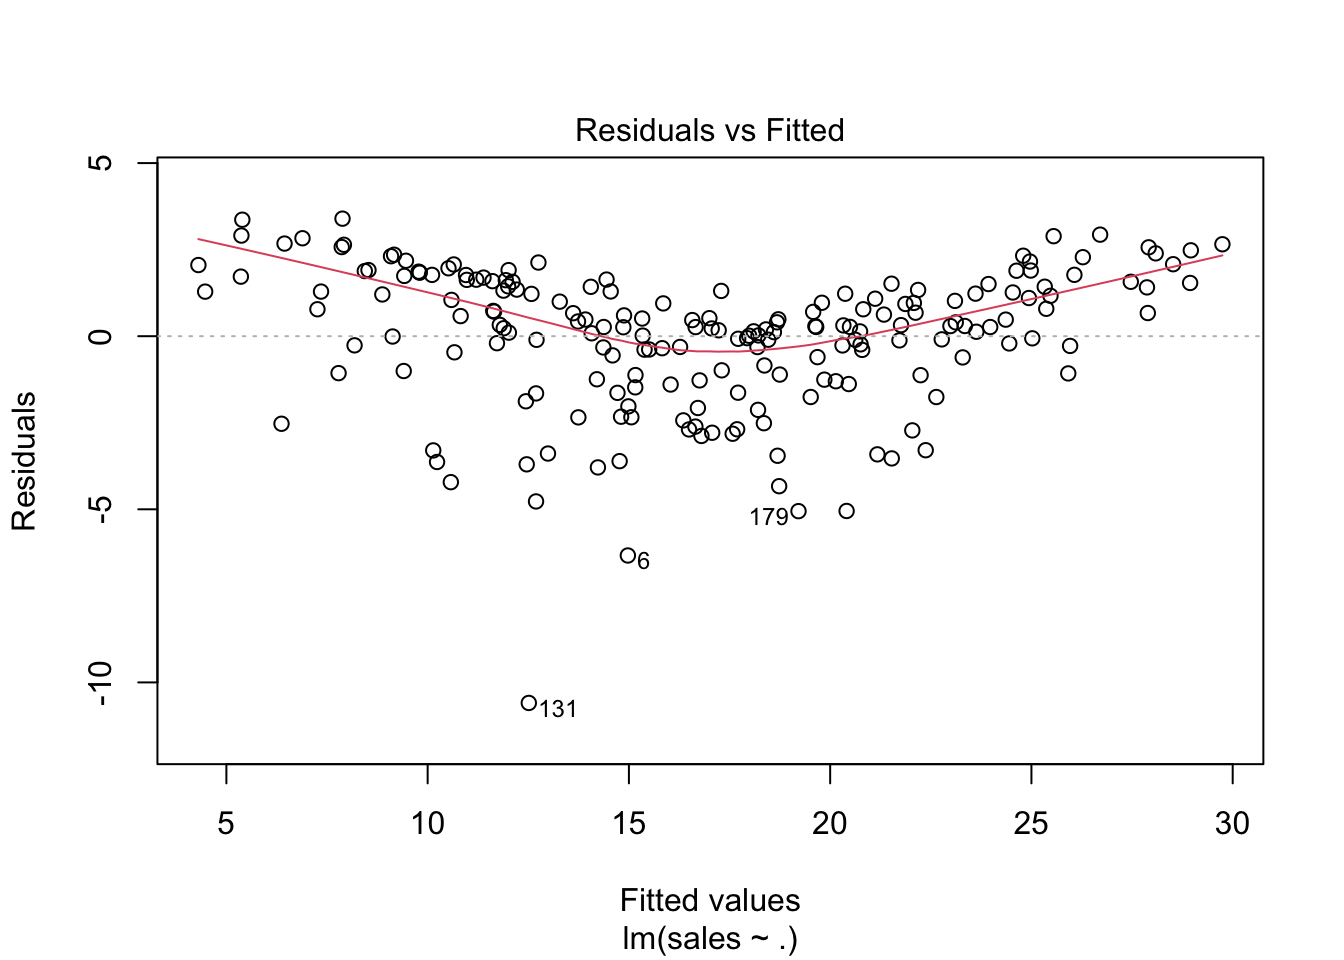
\includegraphics{applied_lecture_notes_files/figure-latex/unnamed-chunk-10-1.pdf}
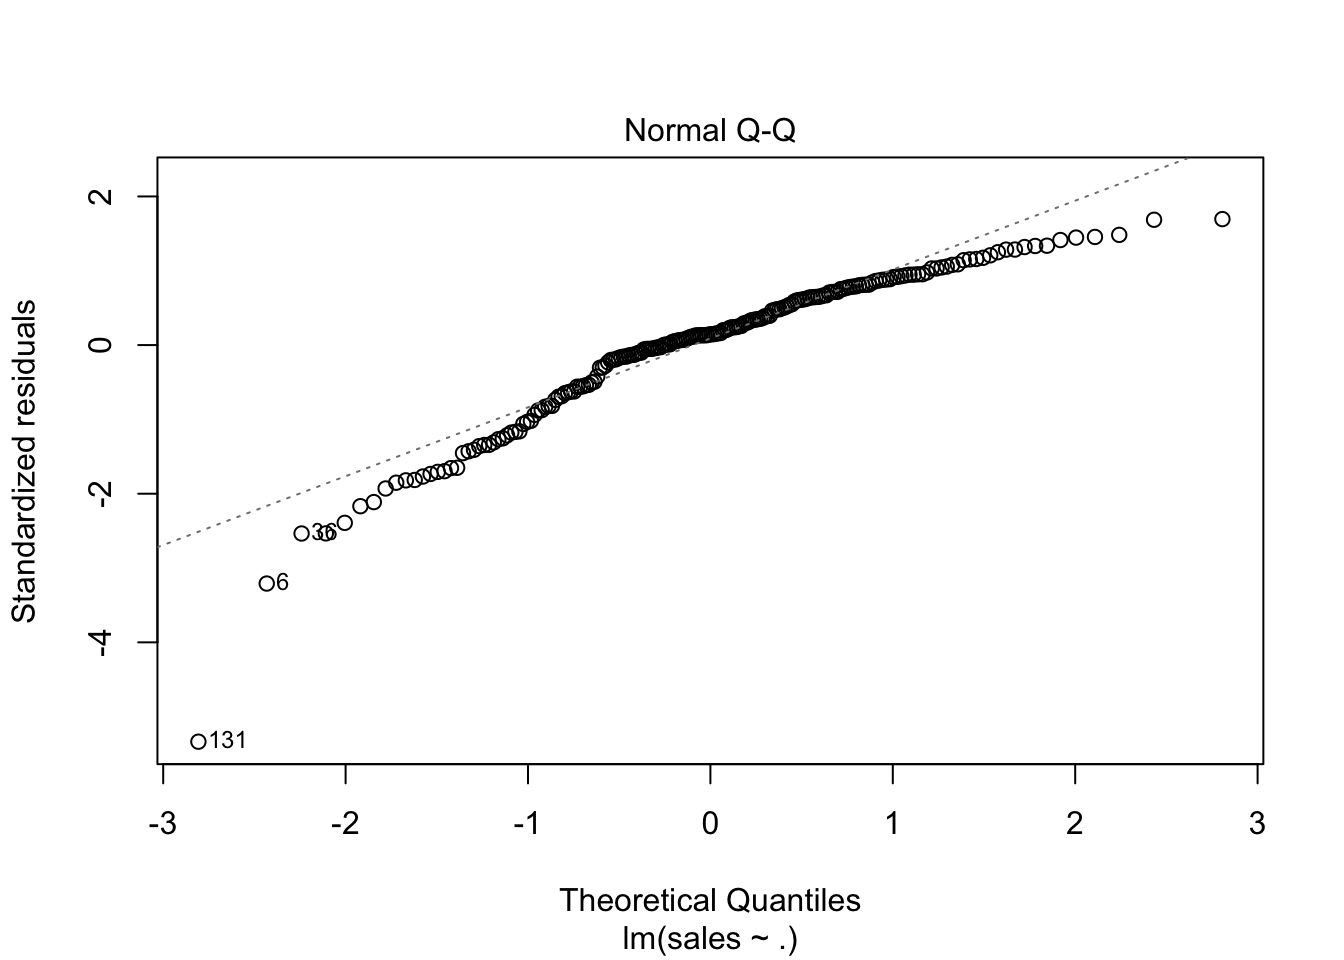
\includegraphics{applied_lecture_notes_files/figure-latex/unnamed-chunk-10-2.pdf}
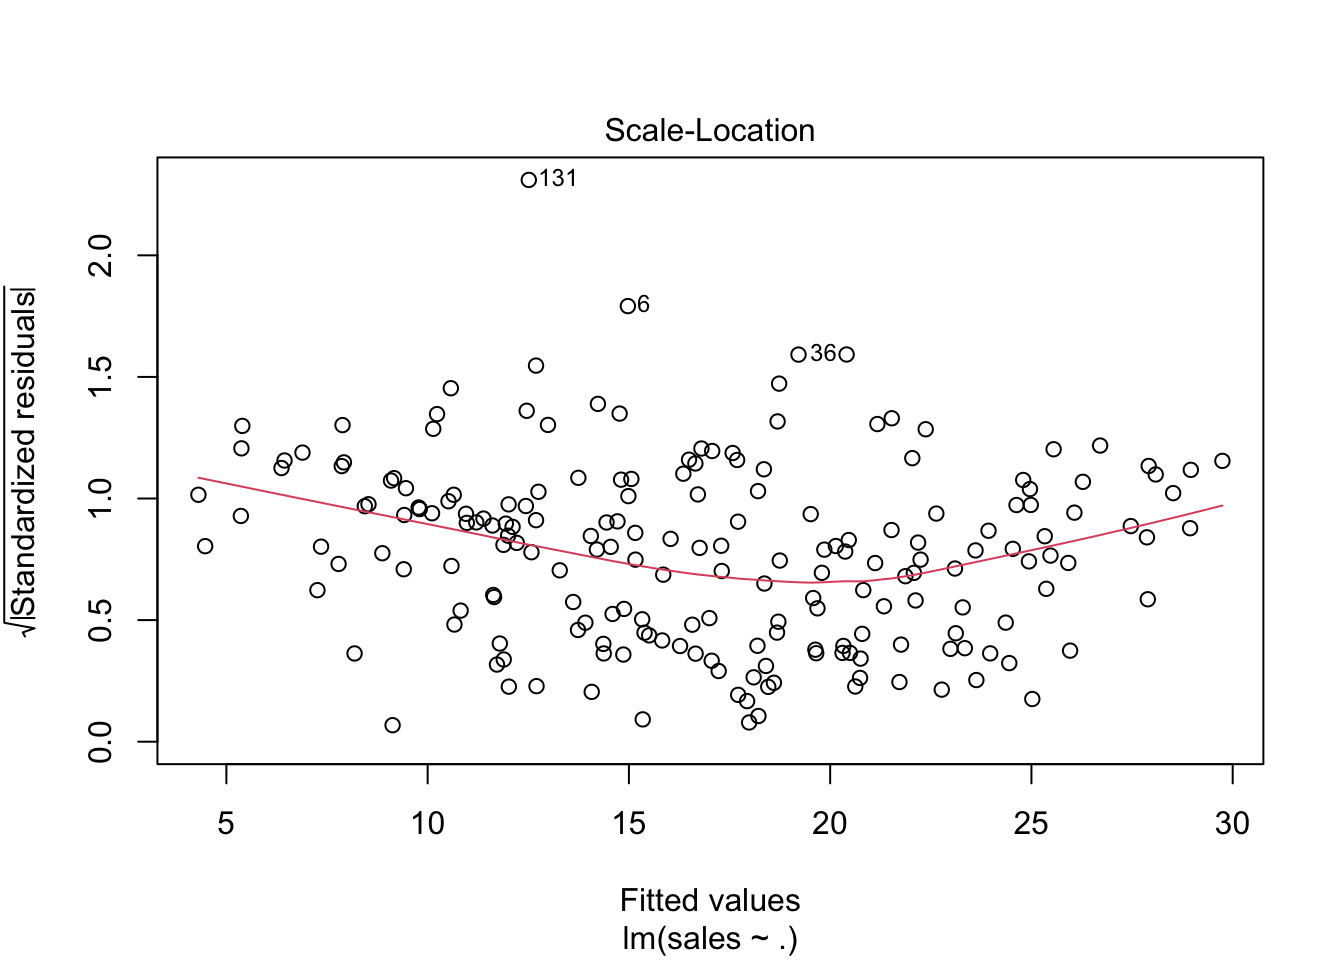
\includegraphics{applied_lecture_notes_files/figure-latex/unnamed-chunk-10-3.pdf}
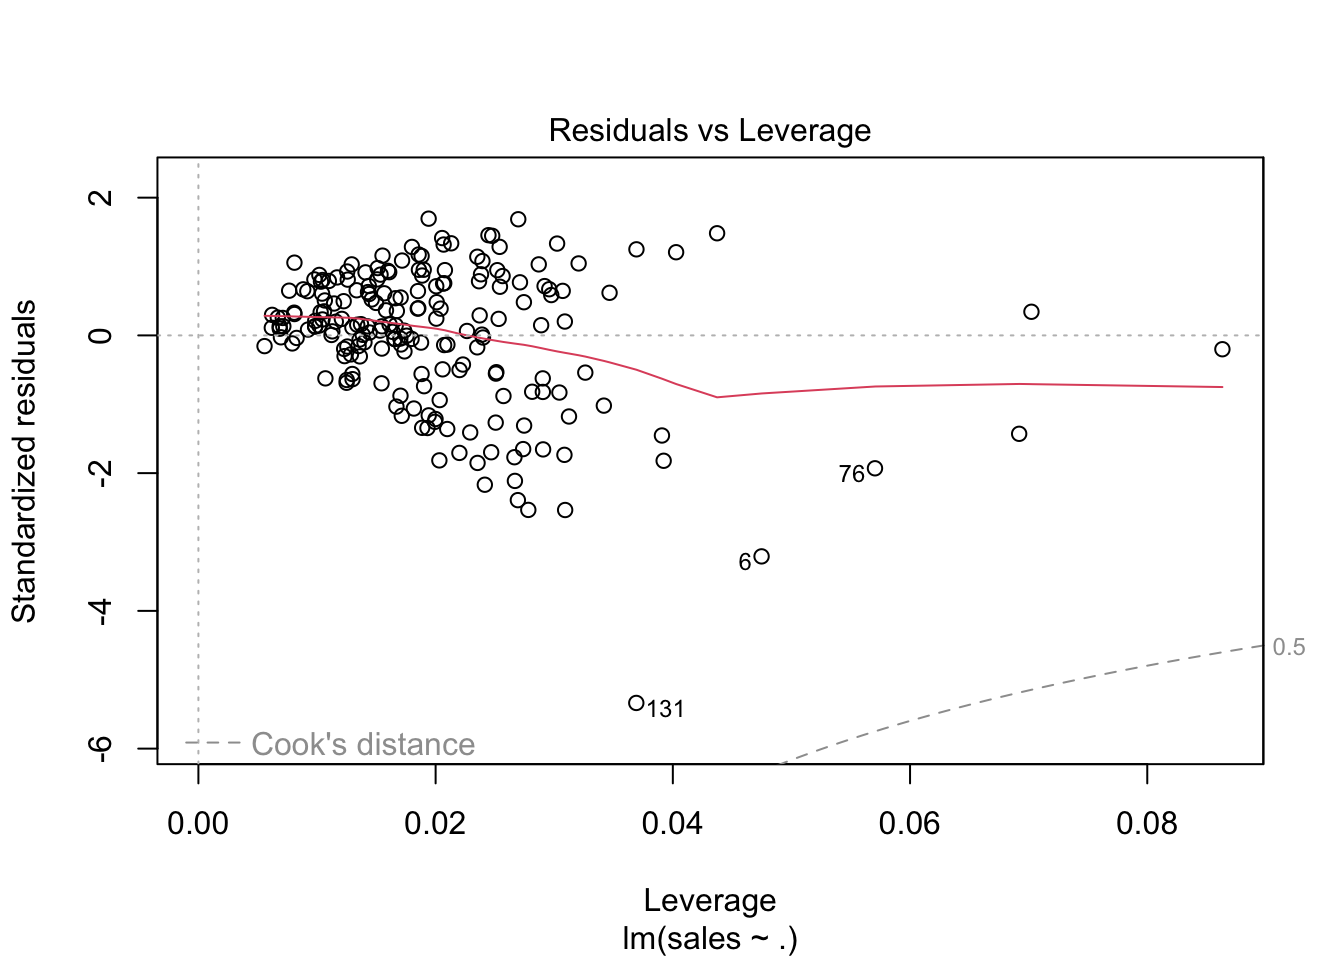
\includegraphics{applied_lecture_notes_files/figure-latex/unnamed-chunk-10-4.pdf}
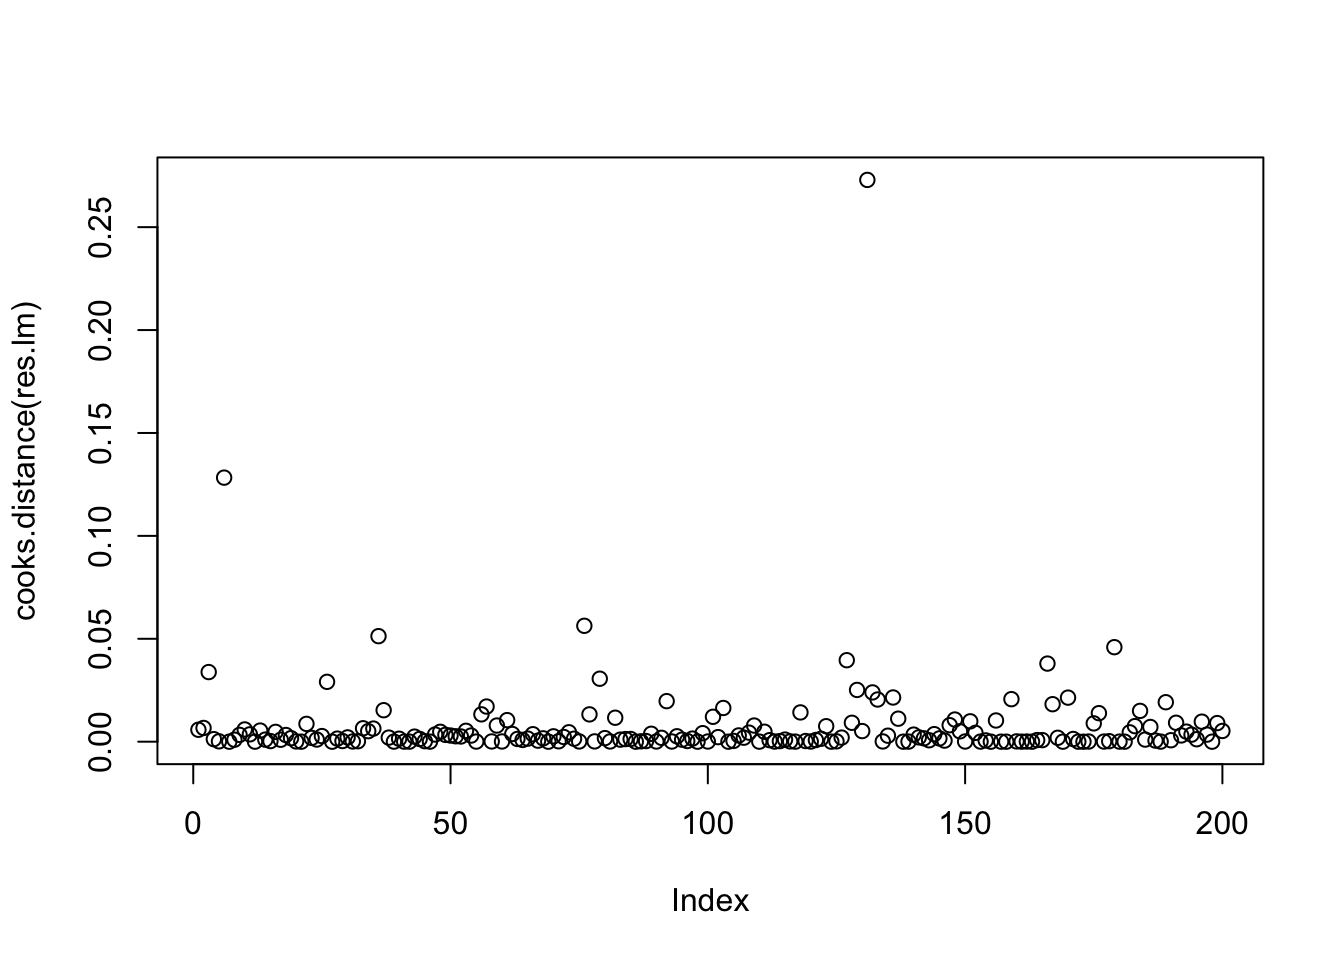
\includegraphics{applied_lecture_notes_files/figure-latex/unnamed-chunk-11-1.pdf}

\hypertarget{handle-outliers}{%
\subsubsection{Handle outliers}\label{handle-outliers}}

-Delete them: be careful, can be sometimes the right thing to do -Change
the model: outliers break a pattern, they may represent a class we're
not fitting, might want to change our model to account for two or
multiple behaviours/populations -Robust linear regression: downsize the
influence of outliers

\hypertarget{partial-correlation}{%
\subsection{Partial correlation}\label{partial-correlation}}

\hypertarget{two-variable-regression}{%
\subsubsection{Two variable regression}\label{two-variable-regression}}

Back to \(Y=\beta X+\gamma Z+\varepsilon\), suppose \(X, Z\) our two
variables. Least square estimate \[
\begin{pmatrix}\hat{\beta}\\\hat{\gamma}\end{pmatrix}=\begin{pmatrix}X^T X & X^T Z\\Z^T X & Z^T Z\end{pmatrix}^{-1}\begin{pmatrix}X^T Y\\X^T Y\end{pmatrix}
\]

Use block matrix inversion, note that \(Z(Z^T Z)^{-1}Z^T\) is a ``hat
matrix'' for regression \(X\) over \(Z\) in the top first of diagonal
matrix, and the RSS in the bottom last.

\[
\begin{pmatrix}X^T X & X^T Z\\Z^T X & Z^T Z\end{pmatrix}^{-1}=\begin{pmatrix}(X^T X) &\\&\end{pmatrix}\times\begin{pmatrix} &\\ &\end{pmatrix}
\]

\hypertarget{two-stage-linear-regression}{%
\subsubsection{Two-stage linear
regression}\label{two-stage-linear-regression}}

We find the exact same result as previously. This is a very useful
trick. Can be extended to multivariate case.

\hypertarget{partial-correlation-and-pairwise-correlation}{%
\subsubsection{Partial correlation and pairwise
correlation}\label{partial-correlation-and-pairwise-correlation}}

See : \url{https://en.wikipedia.org/wiki/Partial_correlation} Do the
computation using slides

If conditional mean is not linear, the conditional correlation is
different from partial correlation.

\hypertarget{geometric-interpretation}{%
\subsubsection{Geometric
interpretation}\label{geometric-interpretation}}

We project \(Y\) to the \(Z\) direction, and the residuals are obtained
as what left in \(r_y\) and similarly for \(X\). The partial correlation
is the angle obtained between those two residuals.

In practice, the simplest is to do a two-stage linear regression and get
the correlation. Another way is to run linear regression of \(Y\) on
\((X,Z)\), however this is not gonna be enough, still need to run \(X\)
on \(Z\) because the coefficient of \(Y\) on \((X,Z)\) is gonna be the
partial correlation \(\times\) a function of the coef of \(X\) on \(Z\)
(compute it by hand to see).

\#Lecture 8 Disclaimer: Exam will be in two parts.

Recap: -Leverage -Standardized residual -Cook's distance -Partial
correlation

\hypertarget{omitted-variable-bias}{%
\subsection{Omitted Variable Bias}\label{omitted-variable-bias}}

We are asking ourselves what influence has missing a variable \(Z\) in
our model. Suppose tue true model \(Y=\rho^T X+\gamma^T Z+\varepsilon\)
but we fit \(Y=X\beta+\varepsilno\).

Recall :

\[\beta=\frac{Cov(X,Y)}{Var(X)}=\frac{Cov(X,\rho^T X+\gamma^T Z)}{Var(X)}\\
=\rho^T+\underbrace_{\text{ommitted variable bias}{\gamma^T\frac{Cov(X,Z)}{Var(X)}}
\]

\hypertarget{toy-example-palmer-station-penguin-data}{%
\subsection{Toy example: Palmer station penguin
data}\label{toy-example-palmer-station-penguin-data}}

\begin{Shaded}
\begin{Highlighting}[]
\FunctionTok{head}\NormalTok{(penguins)}
\end{Highlighting}
\end{Shaded}

\begin{verbatim}
## # A tibble: 6 x 8
##   species island    bill_length_mm bill_depth_mm flipper_l~1 body_~2 sex    year
##   <fct>   <fct>              <dbl>         <dbl>       <int>   <int> <fct> <int>
## 1 Adelie  Torgersen           39.1          18.7         181    3750 male   2007
## 2 Adelie  Torgersen           39.5          17.4         186    3800 fema~  2007
## 3 Adelie  Torgersen           40.3          18           195    3250 fema~  2007
## 4 Adelie  Torgersen           NA            NA            NA      NA <NA>   2007
## 5 Adelie  Torgersen           36.7          19.3         193    3450 fema~  2007
## 6 Adelie  Torgersen           39.3          20.6         190    3650 male   2007
## # ... with abbreviated variable names 1: flipper_length_mm, 2: body_mass_g
\end{verbatim}

\begin{Shaded}
\begin{Highlighting}[]
\FunctionTok{plot}\NormalTok{(penguins}\SpecialCharTok{$}\NormalTok{bill\_length\_mm, penguins}\SpecialCharTok{$}\NormalTok{bill\_depth\_mm, }\AttributeTok{pch=}\DecValTok{19}\NormalTok{)}
\end{Highlighting}
\end{Shaded}

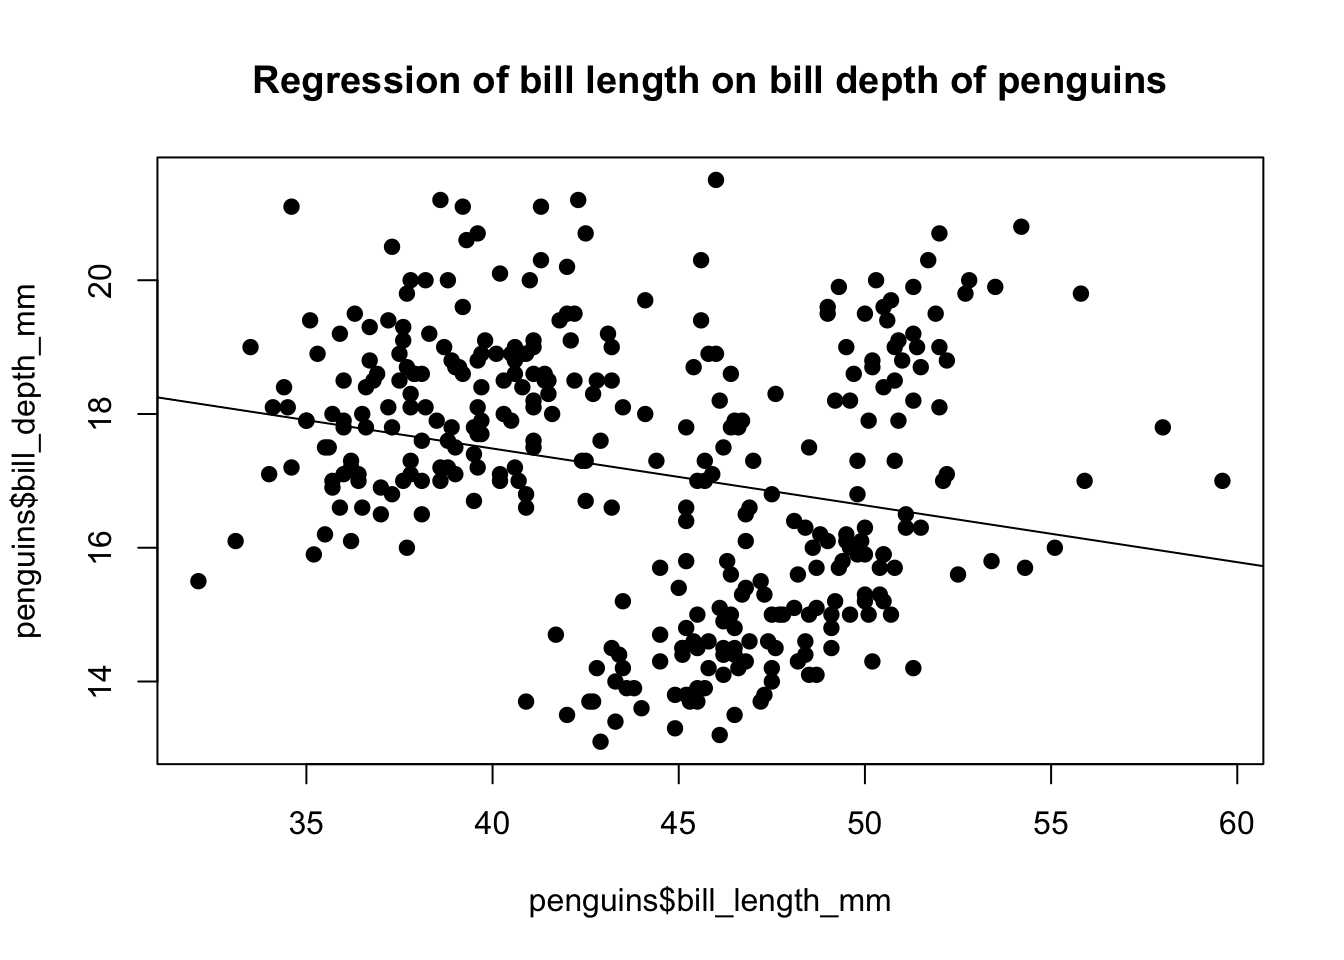
\includegraphics{applied_lecture_notes_files/figure-latex/unnamed-chunk-13-1.pdf}

\begin{Shaded}
\begin{Highlighting}[]
\NormalTok{lin\_reg }\OtherTok{\textless{}{-}}\FunctionTok{lm}\NormalTok{(bill\_depth\_mm }\SpecialCharTok{\textasciitilde{}}\NormalTok{bill\_length\_mm, }\AttributeTok{data=}\NormalTok{penguins)}
\FunctionTok{summary}\NormalTok{(lin\_reg)}
\end{Highlighting}
\end{Shaded}

\begin{verbatim}
## 
## Call:
## lm(formula = bill_depth_mm ~ bill_length_mm, data = penguins)
## 
## Residuals:
##     Min      1Q  Median      3Q     Max 
## -4.1381 -1.4263  0.0164  1.3841  4.5255 
## 
## Coefficients:
##                Estimate Std. Error t value Pr(>|t|)    
## (Intercept)    20.88547    0.84388  24.749  < 2e-16 ***
## bill_length_mm -0.08502    0.01907  -4.459 1.12e-05 ***
## ---
## Signif. codes:  0 '***' 0.001 '**' 0.01 '*' 0.05 '.' 0.1 ' ' 1
## 
## Residual standard error: 1.922 on 340 degrees of freedom
##   (2 observations effacées parce que manquantes)
## Multiple R-squared:  0.05525,    Adjusted R-squared:  0.05247 
## F-statistic: 19.88 on 1 and 340 DF,  p-value: 1.12e-05
\end{verbatim}

This looks ``fine'' in numbers\ldots{} What is the issue here ? We're
confronted to a \emph{Simpson paradox}.

What about our diagnostics ? The residuals vs fitted are slightly
worrying, the fit is not perfect but nonetheless the linear relationship
seems to be reasonable.

\begin{Shaded}
\begin{Highlighting}[]
\FunctionTok{plot}\NormalTok{(penguins}\SpecialCharTok{$}\NormalTok{bill\_length\_mm, penguins}\SpecialCharTok{$}\NormalTok{bill\_depth\_mm, }\AttributeTok{pch=}\DecValTok{19}\NormalTok{, }\AttributeTok{main=}\StringTok{"Regression of bill length on bill depth of penguins"}\NormalTok{)}
\FunctionTok{abline}\NormalTok{(}\FunctionTok{coef}\NormalTok{(lin\_reg))}
\end{Highlighting}
\end{Shaded}

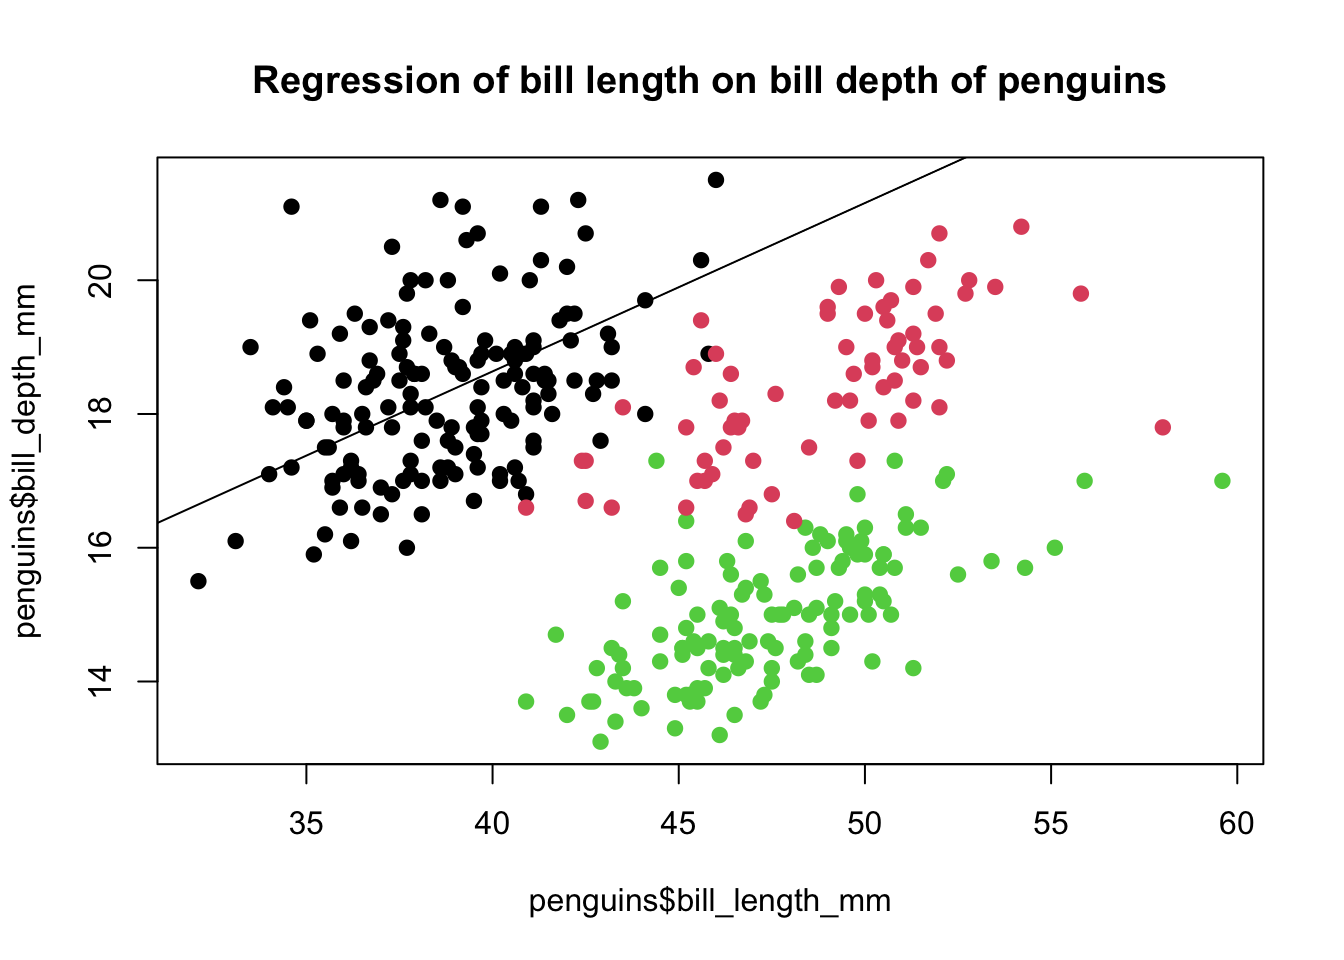
\includegraphics{applied_lecture_notes_files/figure-latex/unnamed-chunk-15-1.pdf}

\begin{Shaded}
\begin{Highlighting}[]
\FunctionTok{plot}\NormalTok{(lin\_reg)}
\end{Highlighting}
\end{Shaded}

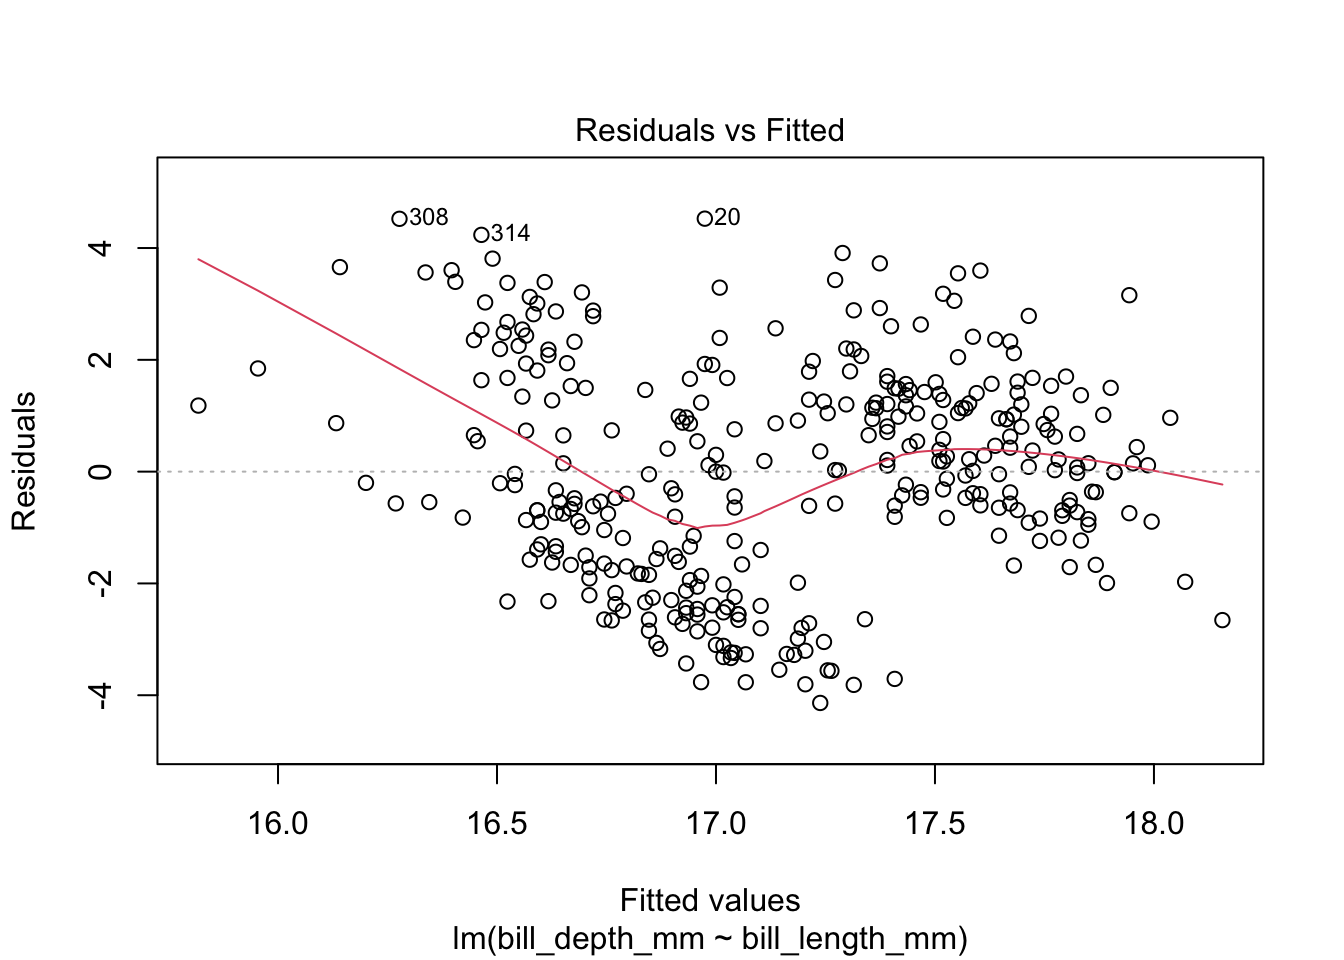
\includegraphics{applied_lecture_notes_files/figure-latex/unnamed-chunk-15-2.pdf}
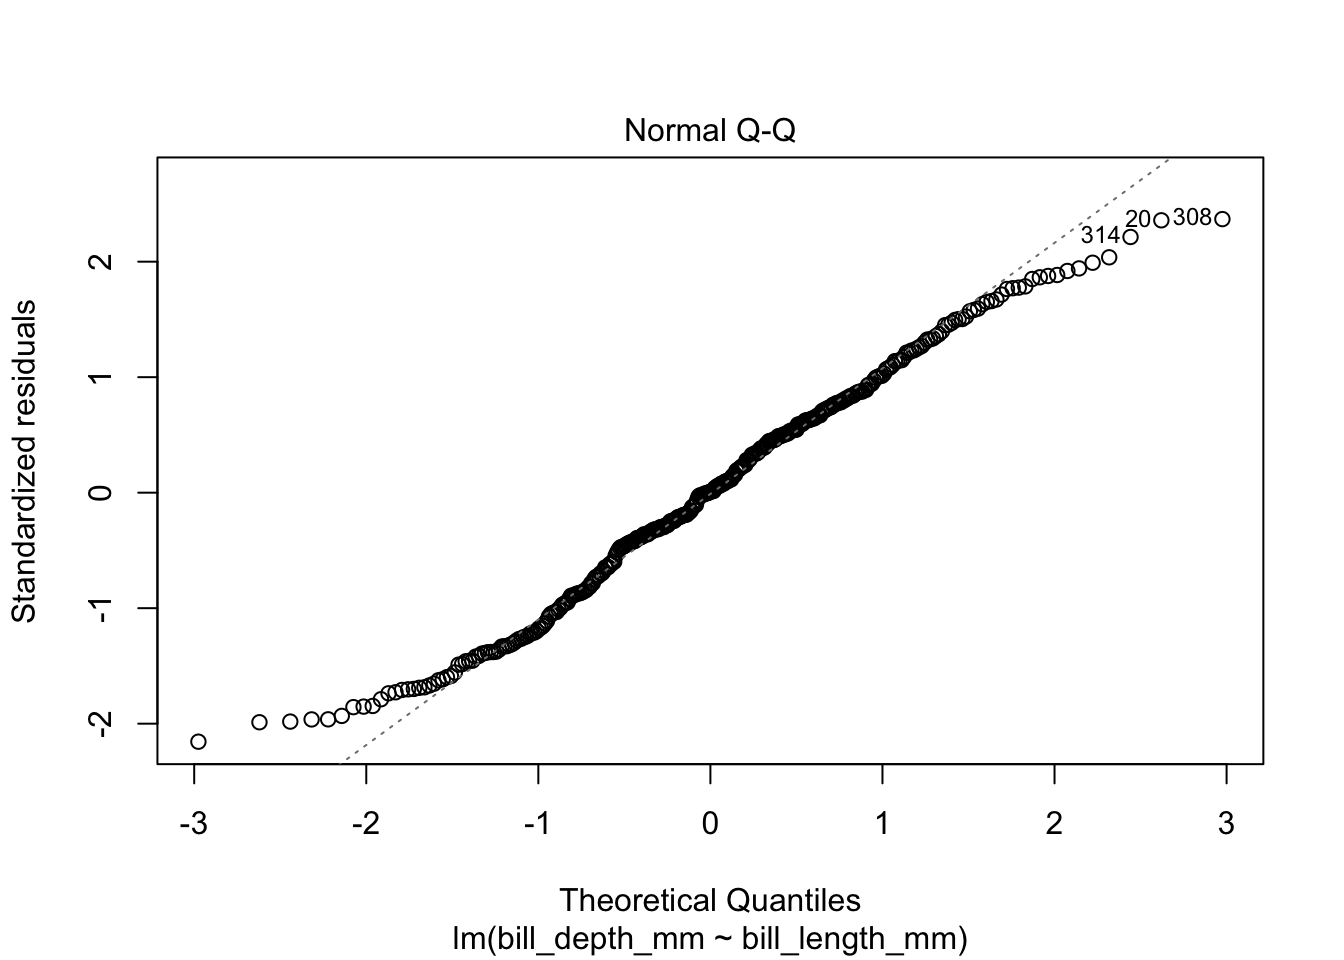
\includegraphics{applied_lecture_notes_files/figure-latex/unnamed-chunk-15-3.pdf}
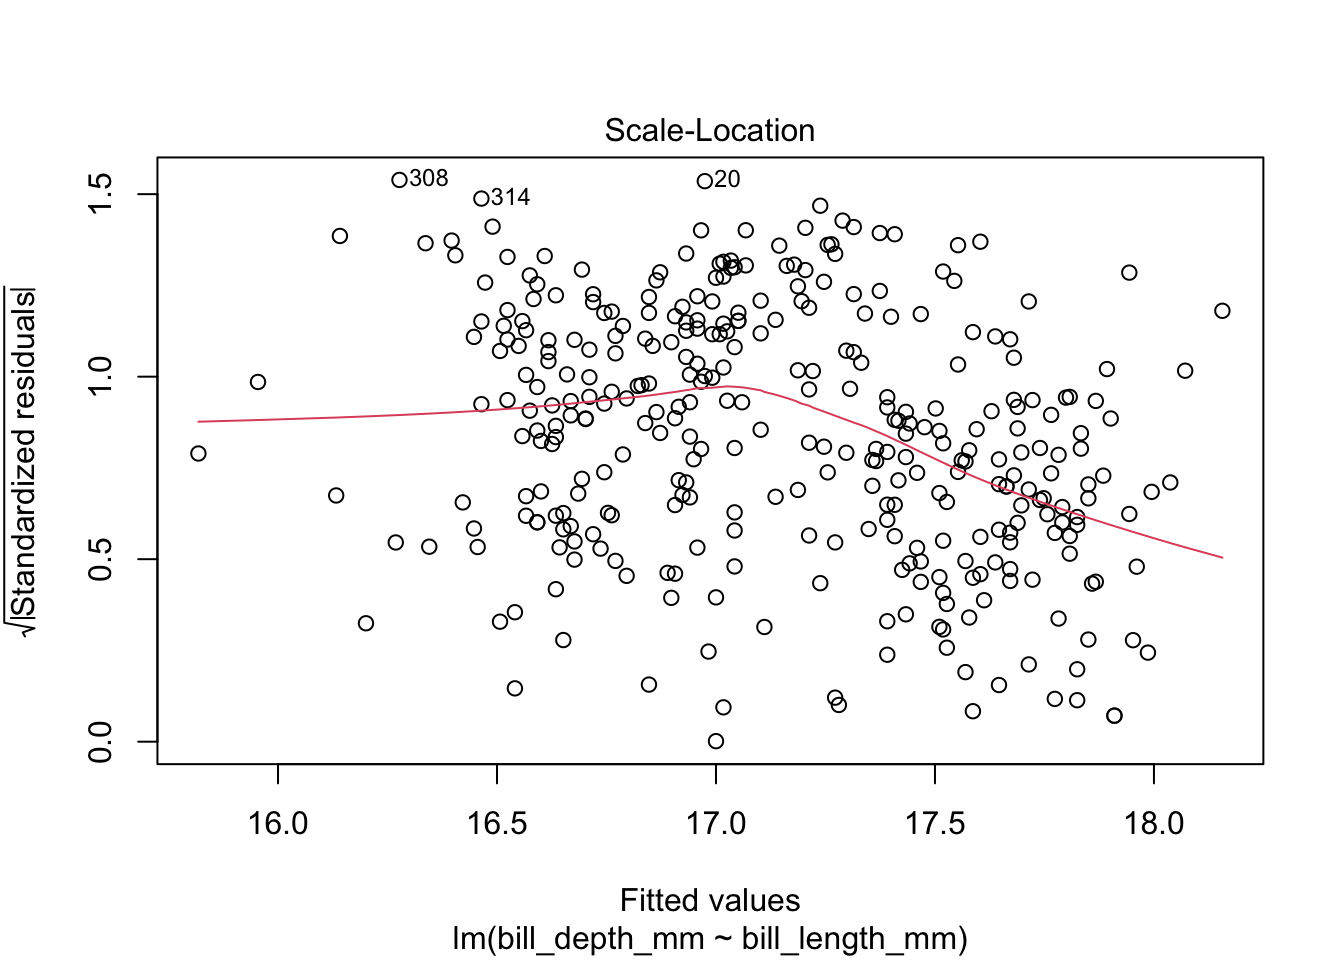
\includegraphics{applied_lecture_notes_files/figure-latex/unnamed-chunk-15-4.pdf}
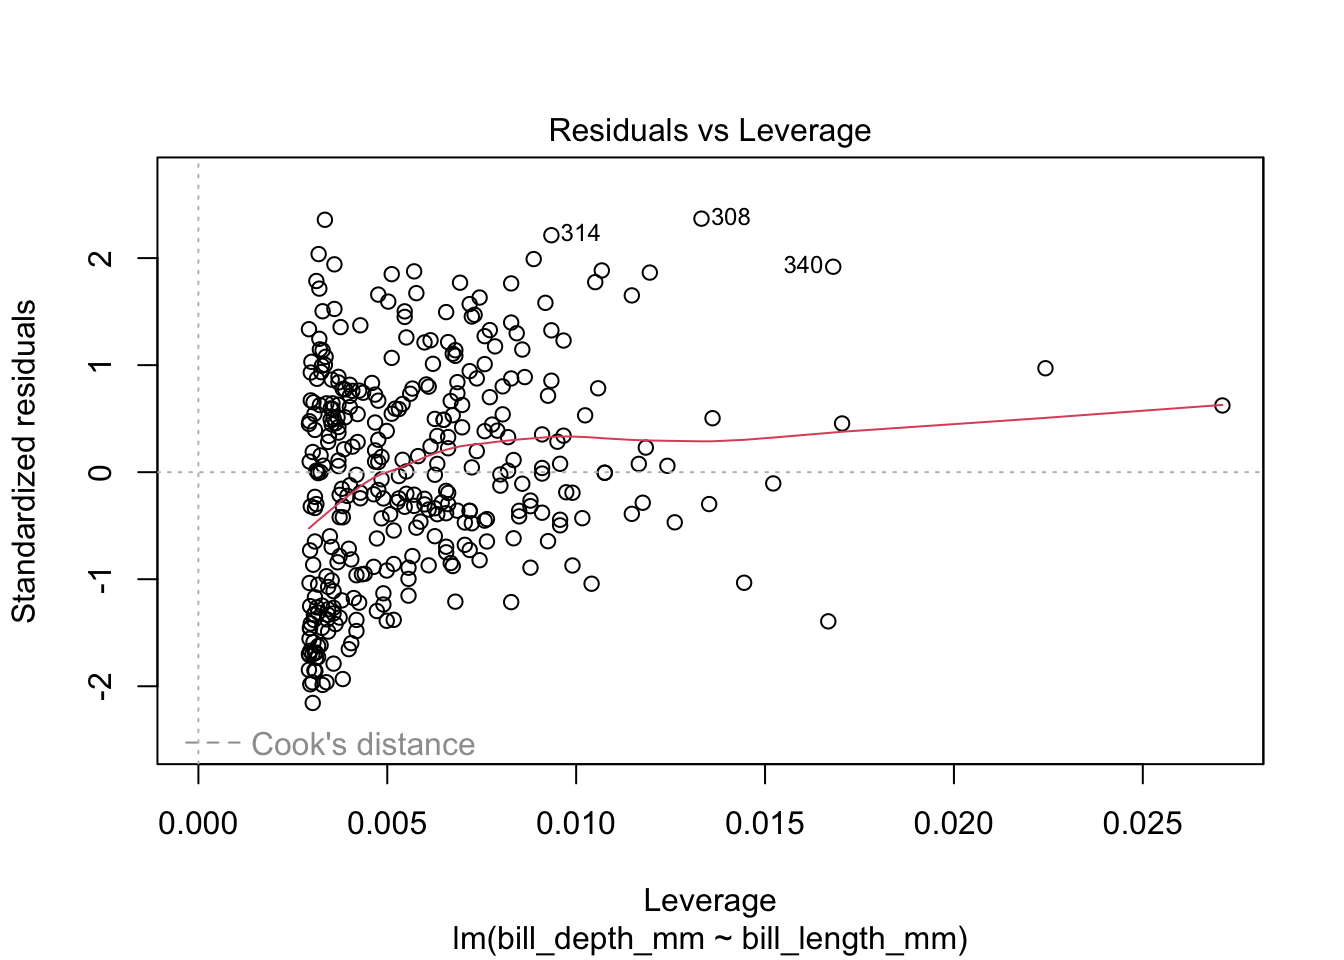
\includegraphics{applied_lecture_notes_files/figure-latex/unnamed-chunk-15-5.pdf}

How do we interpret this result ? The longer the beak, the shallower it
is. This sounds silly. We can sense the problem of our regression on the
residual vs fitted plot. There are two stacks of point around the
\(x\)s, we can see two or more ``clumps''\ldots{} What is missing is the
variable of species !

\begin{Shaded}
\begin{Highlighting}[]
\NormalTok{lin\_1 }\OtherTok{\textless{}{-}}\FunctionTok{lm}\NormalTok{(bill\_depth\_mm }\SpecialCharTok{\textasciitilde{}}\NormalTok{bill\_length\_mm}\SpecialCharTok{:}\NormalTok{ species, }\AttributeTok{data=}\NormalTok{penguins)}
\FunctionTok{summary}\NormalTok{(lin\_1)}
\end{Highlighting}
\end{Shaded}

\begin{verbatim}
## 
## Call:
## lm(formula = bill_depth_mm ~ bill_length_mm:species, data = penguins)
## 
## Residuals:
##     Min      1Q  Median      3Q     Max 
## -2.4763 -0.7151 -0.0558  0.5865  3.8226 
## 
## Coefficients:
##                                 Estimate Std. Error t value Pr(>|t|)    
## (Intercept)                      8.56283    0.78487   10.91  < 2e-16 ***
## bill_length_mm:speciesAdelie     0.25187    0.02024   12.44  < 2e-16 ***
## bill_length_mm:speciesChinstrap  0.20196    0.01618   12.48  < 2e-16 ***
## bill_length_mm:speciesGentoo     0.13542    0.01656    8.18 5.83e-15 ***
## ---
## Signif. codes:  0 '***' 0.001 '**' 0.01 '*' 0.05 '.' 0.1 ' ' 1
## 
## Residual standard error: 0.9699 on 338 degrees of freedom
##   (2 observations effacées parce que manquantes)
## Multiple R-squared:  0.7609, Adjusted R-squared:  0.7588 
## F-statistic: 358.6 on 3 and 338 DF,  p-value: < 2.2e-16
\end{verbatim}

\begin{Shaded}
\begin{Highlighting}[]
\FunctionTok{plot}\NormalTok{(lin\_1)}
\end{Highlighting}
\end{Shaded}

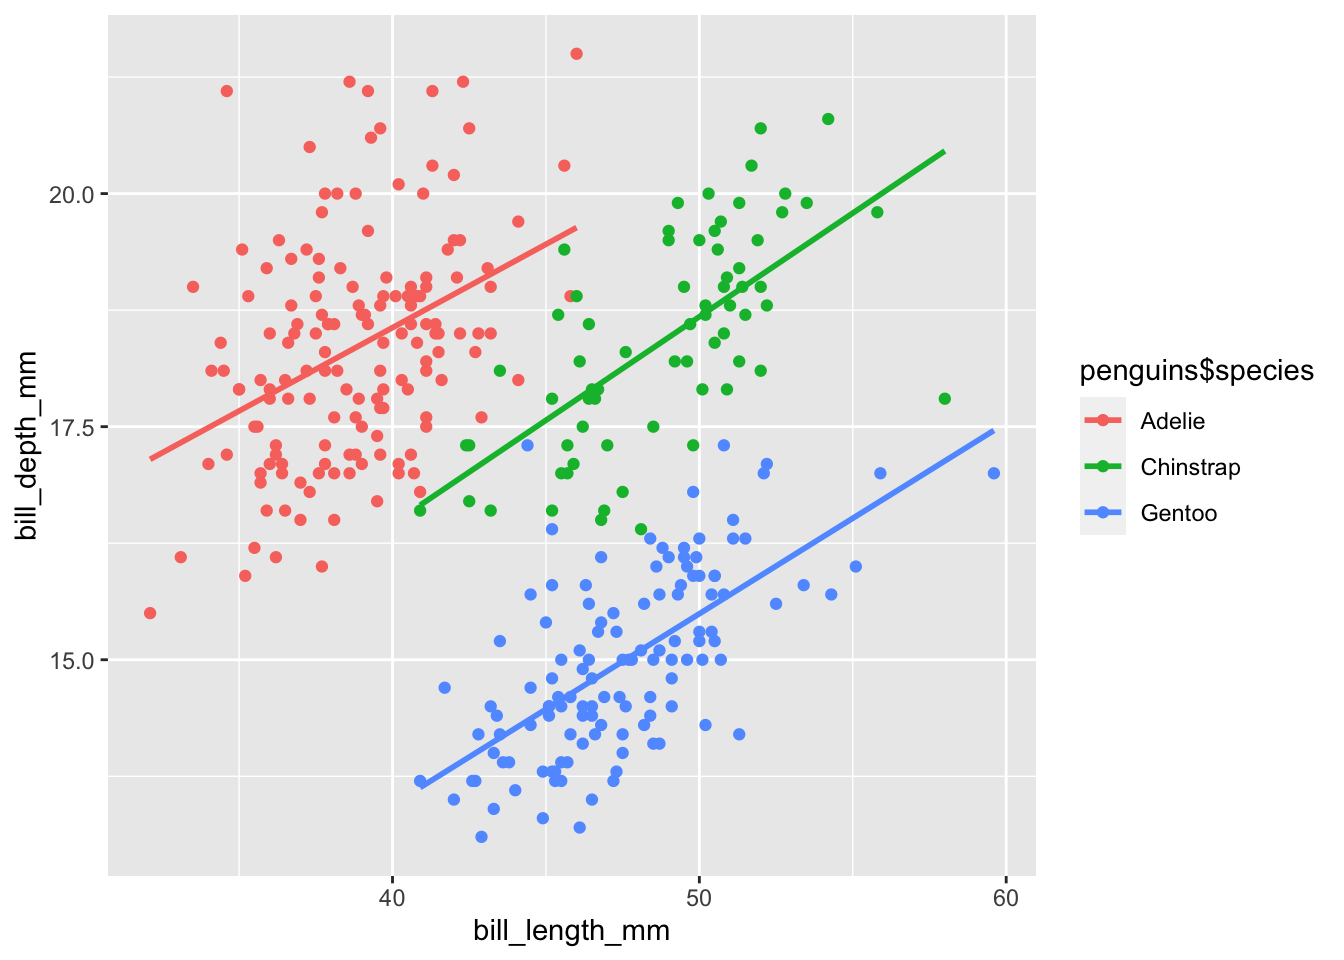
\includegraphics{applied_lecture_notes_files/figure-latex/unnamed-chunk-16-1.pdf}
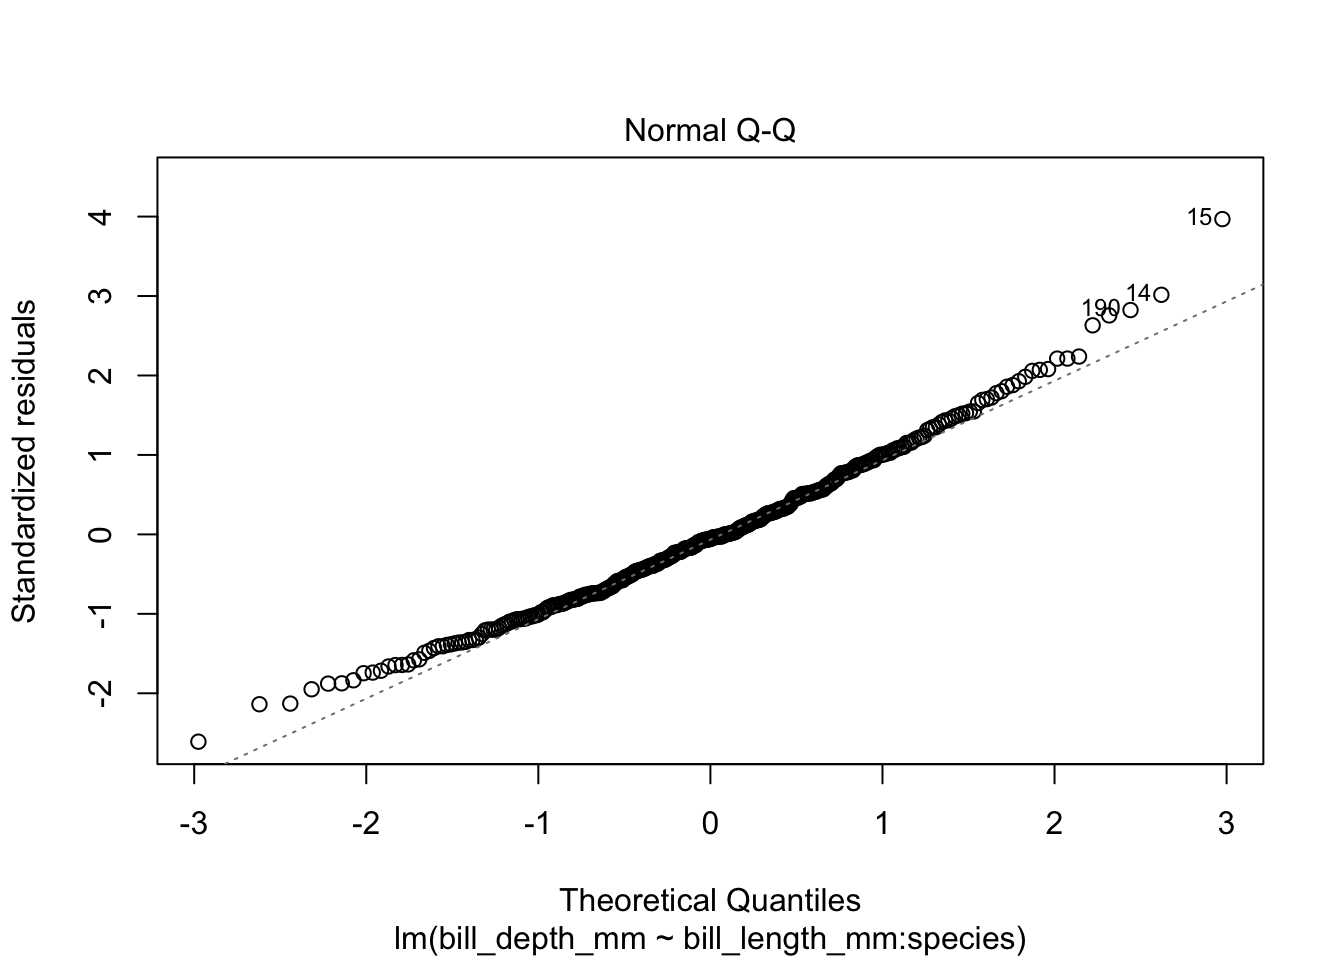
\includegraphics{applied_lecture_notes_files/figure-latex/unnamed-chunk-16-2.pdf}
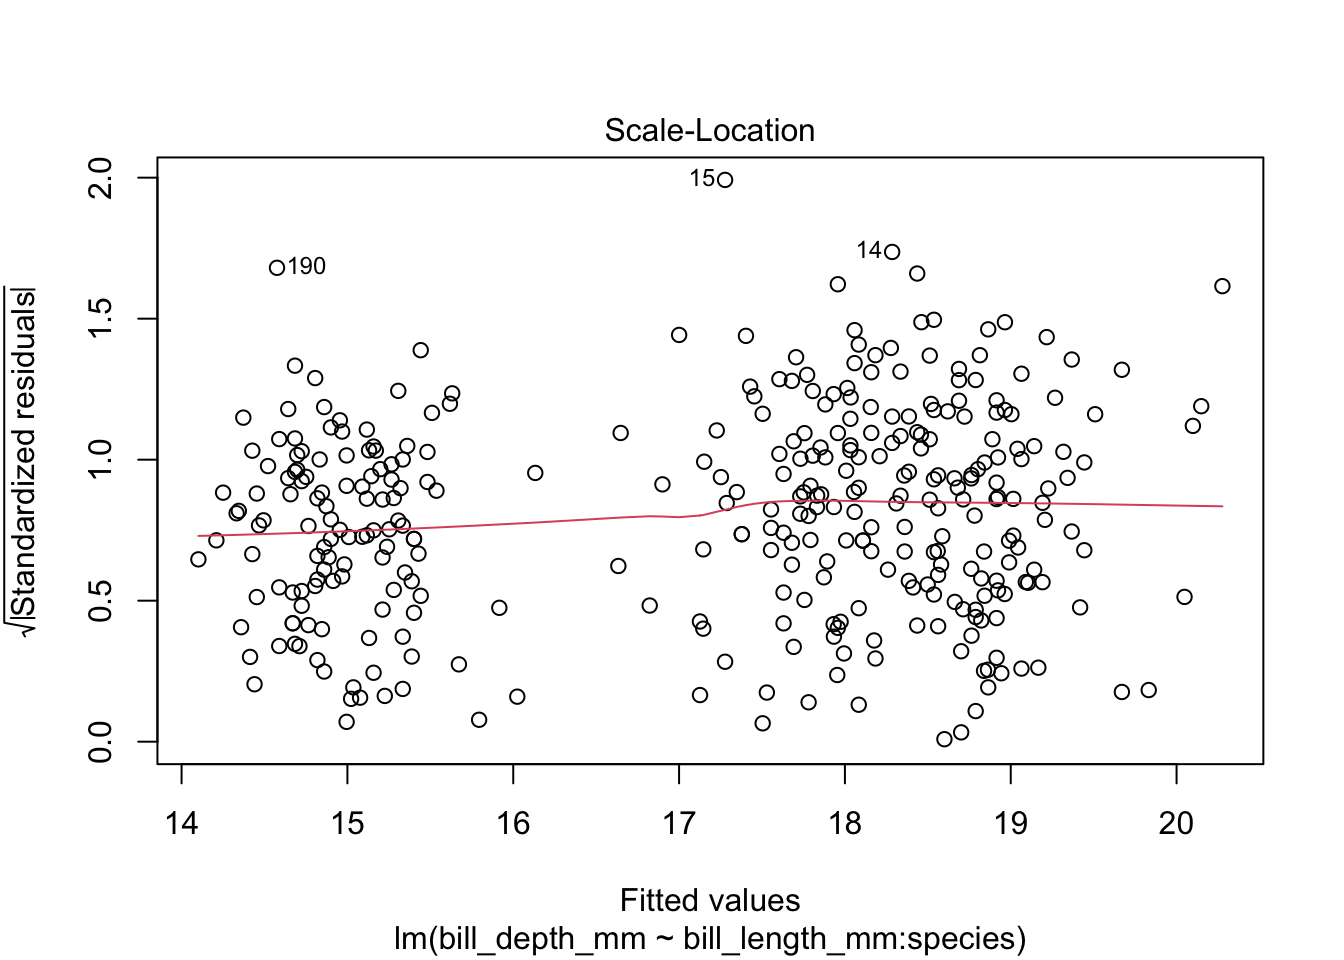
\includegraphics{applied_lecture_notes_files/figure-latex/unnamed-chunk-16-3.pdf}
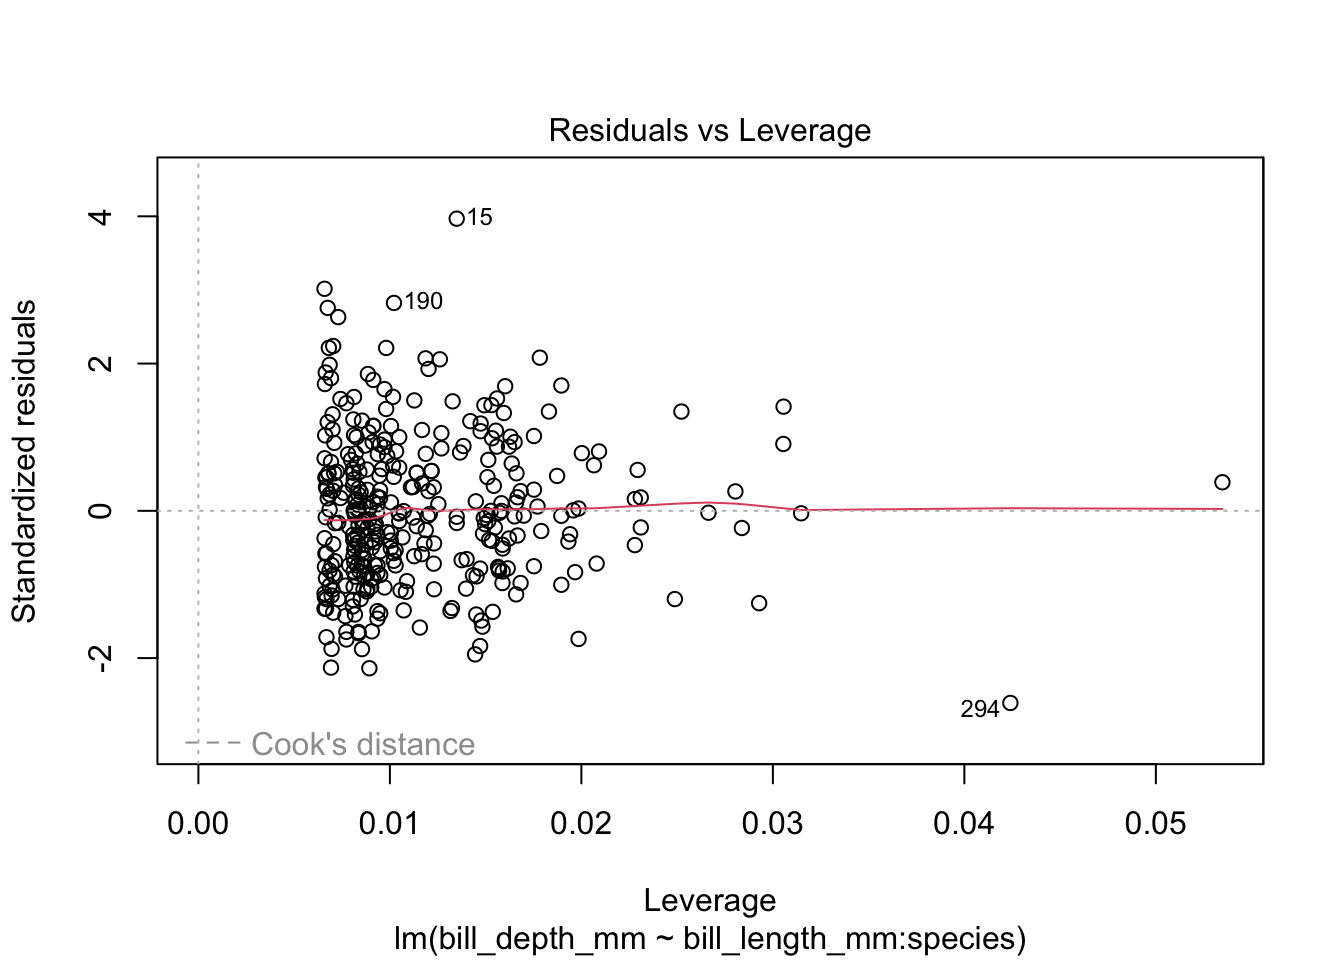
\includegraphics{applied_lecture_notes_files/figure-latex/unnamed-chunk-16-4.pdf}

\begin{Shaded}
\begin{Highlighting}[]
\FunctionTok{plot}\NormalTok{(penguins}\SpecialCharTok{$}\NormalTok{bill\_length\_mm, penguins}\SpecialCharTok{$}\NormalTok{bill\_depth\_mm, }\AttributeTok{col=}\NormalTok{penguins}\SpecialCharTok{$}\NormalTok{species, }\AttributeTok{pch=}\DecValTok{19}\NormalTok{, }\AttributeTok{main=}\StringTok{"Regression of bill length on bill depth of penguins"}\NormalTok{)}
\NormalTok{a}\OtherTok{=}\FloatTok{8.5628281}
\NormalTok{Adelie}\OtherTok{=}\FloatTok{0.2518668}
\NormalTok{Chinstrap}\OtherTok{=}\FloatTok{0.2019567}
\NormalTok{Gentoo}\OtherTok{=}\FloatTok{0.2518668}
\FunctionTok{abline}\NormalTok{(}\AttributeTok{a=}\FunctionTok{c}\NormalTok{(a,a,a), }\AttributeTok{b=}\FunctionTok{c}\NormalTok{(Adelie, Chinstrap, Gentoo), }\AttributeTok{col=}\FunctionTok{c}\NormalTok{(}\StringTok{\textquotesingle{}black\textquotesingle{}}\NormalTok{, }\StringTok{\textquotesingle{}lightpink\textquotesingle{}}\NormalTok{,}\StringTok{\textquotesingle{}green\textquotesingle{}}\NormalTok{))}
\end{Highlighting}
\end{Shaded}

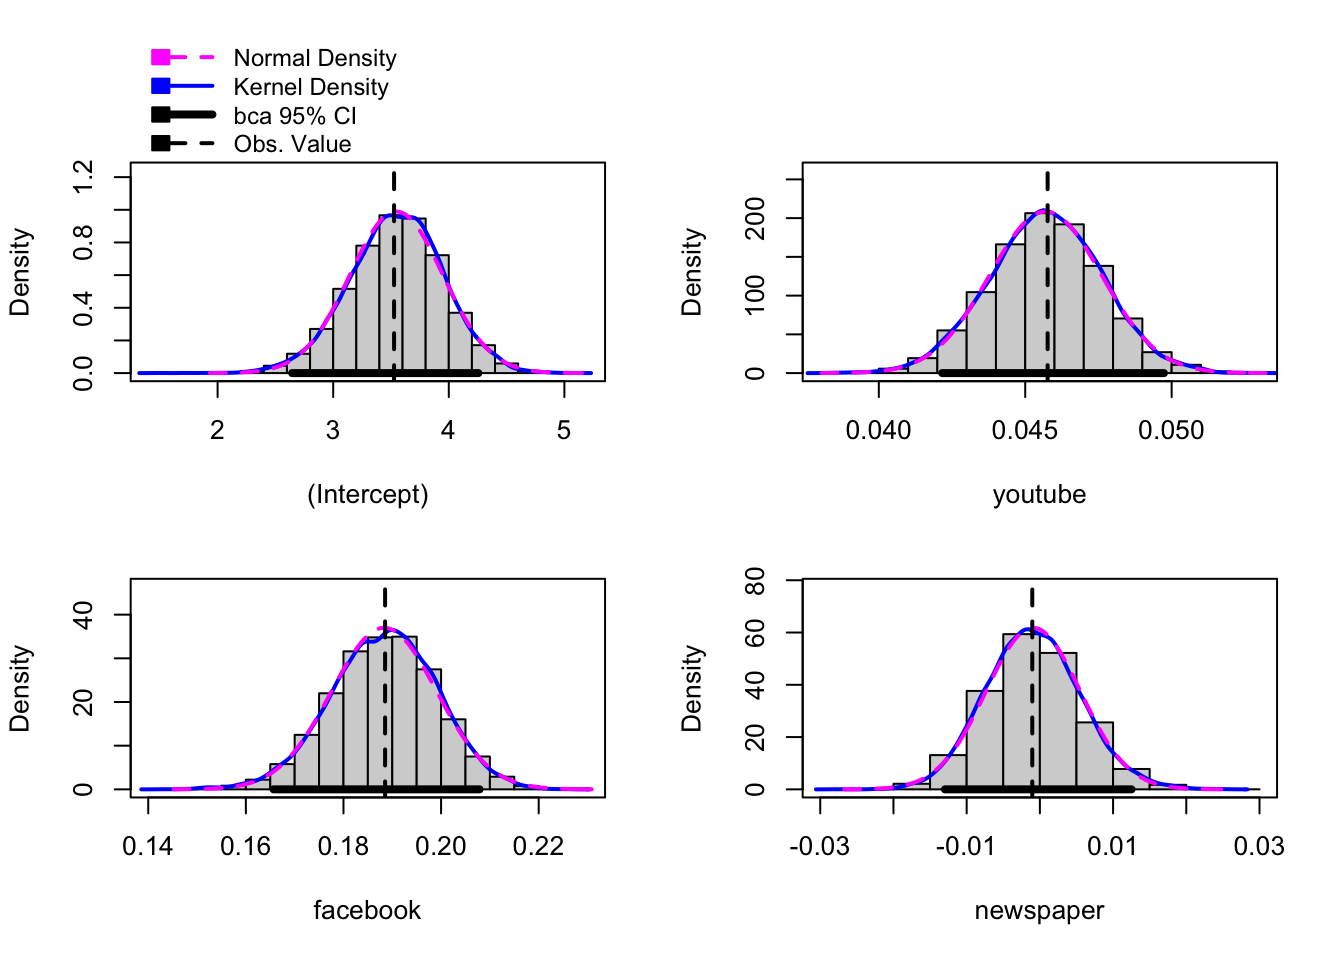
\includegraphics{applied_lecture_notes_files/figure-latex/unnamed-chunk-17-1.pdf}

\begin{Shaded}
\begin{Highlighting}[]
\FunctionTok{ggplot}\NormalTok{(penguins,}\FunctionTok{aes}\NormalTok{(bill\_length\_mm, bill\_depth\_mm, }\AttributeTok{colour=}\NormalTok{penguins}\SpecialCharTok{$}\NormalTok{species))}\SpecialCharTok{+}\FunctionTok{geom\_point}\NormalTok{()}\SpecialCharTok{+}\FunctionTok{geom\_smooth}\NormalTok{(}\AttributeTok{method=}\StringTok{"lm"}\NormalTok{, }\AttributeTok{se=}\ConstantTok{FALSE}\NormalTok{)}
\end{Highlighting}
\end{Shaded}

\begin{verbatim}
## Warning: Use of `penguins$species` is discouraged. Use `species` instead.
## Use of `penguins$species` is discouraged. Use `species` instead.
\end{verbatim}

\begin{verbatim}
## `geom_smooth()` using formula 'y ~ x'
\end{verbatim}

\begin{verbatim}
## Warning: Removed 2 rows containing non-finite values (stat_smooth).
\end{verbatim}

\begin{verbatim}
## Warning: Removed 2 rows containing missing values (geom_point).
\end{verbatim}

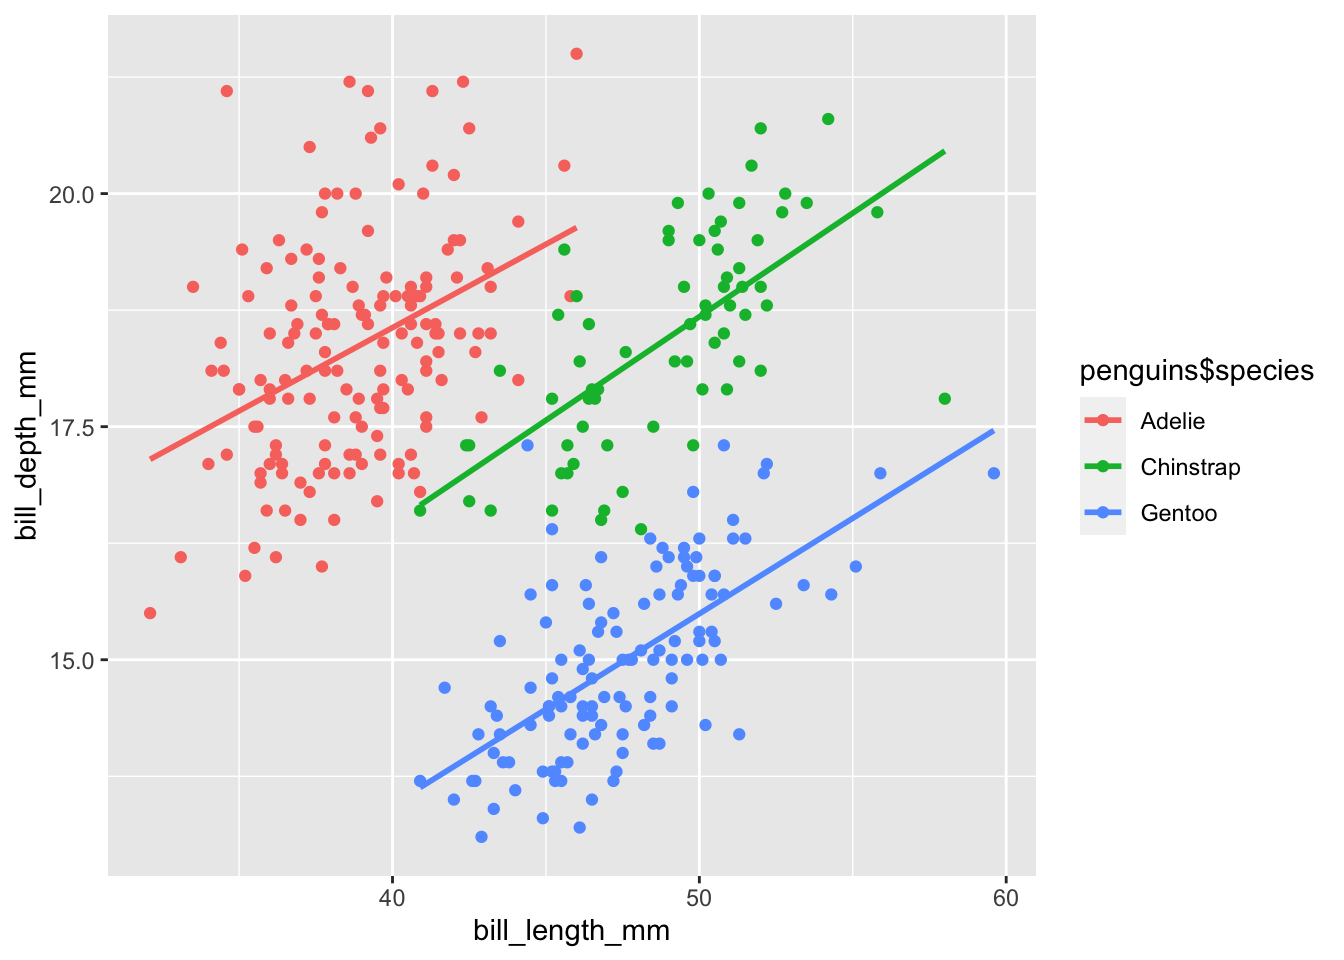
\includegraphics{applied_lecture_notes_files/figure-latex/unnamed-chunk-18-1.pdf}

For each species, the correlation of those two variables is positive,
but for the clumped model, it is negative (which is not really
interpretable)!

\hypertarget{bootstrap}{%
\subsection{Bootstrap}\label{bootstrap}}

\hypertarget{jacknife-estimate}{%
\subsubsection{Jacknife estimate}\label{jacknife-estimate}}

Robust inference under resampling ?

If we look at \(\bar{X}\) from \(X_1,\dots, X_n\), we need to make
assumption about the distribution Now, we replicate this but leaving one
out to have not only one estimate but a population of estimate:
\(\bar{X}_{(-i)}=\frac{1}{n-1}\sum_{j\neq i}X_i\). We don't need an
assumption on the distribution of those objects now, we now have \(n\)
of these objects and we can take as estimate
\(\bar{\bar{X}}=\frac{1}{n}\sum\bar{X}_{(-i)}\).

Variance? Note that all \(\bar{X}_{(-i)}\) are highly correlated, taking
\(\frac{1}{n-1}\sum (\bar{X}_{(-i)}-\bar{\bar{X}})^2\) won't yield the
right amount. Instead, take
\(\frac{n}{n-1}(\bar{X}_{(-i)}-\bar{\bar{X}})^2=\frac{1}{n(n-1)}\sum (X_i-\bar{X})^2\).

Now let's take the model \(Y=X^T\beta+\epsilon\) with
\((X_i, Y_i)_{i=1,\dots, n}\). We compute likewise
\(\hat{\beta}_{(-i)}\) by regression \(Y\) on \(X_{(-i)}\). Computations
yield
\(\hat{\beta}_{(-i)}=(X_{(-i)}^TX_{(-i)})^{-1}X_{(-i)}^T Y_{(-i)}\). A
simple way to retrieve this result with intuition is using the
``leave-one-out'' lemma.that gives
\(\hat{\beta}_{(-i)}=(X^T X)^{-1}X^T\hat{y}_{(-i)}\)

Variance? In the specific case where we already have \(\hat{\beta}\) to
plug in our leave-one-out,
\[\sum_{i=1}^n (\hat{\beta}_{(-i)}-\hat{\beta})(\hat{\beta}_{(-i)}-\hat{\beta})^T 
=(X^TX)^{-1}X^T(\sum (\hat{y}_{(-j)}-(\frac{n-1}{n}y+\frac{1}{n}X^T\hat{\beta})(\hat{y}_{(-j)}-(\frac{n-1}{n}y+\frac{1}{n}X^T\hat{\beta})^T))\\
=(X^T X)X^T D(r_i^2) X(X^T X)^{-1}\]

Downsize: need either a number of regressions\ldots{} if not in this
specific case (in which we can use our closed form formula). Plus:
resample eases inference.

\hypertarget{confidence-interval}{%
\subsubsection{Confidence interval}\label{confidence-interval}}

Point estimate might not be changed by lack of assumptions. However, you
need the assumptions for confidence interval.

\hypertarget{case-resampling}{%
\subsubsection{Case resampling}\label{case-resampling}}

default method of resampling.

\begin{Shaded}
\begin{Highlighting}[]
\NormalTok{fit }\OtherTok{\textless{}{-}}\FunctionTok{lm}\NormalTok{(sales }\SpecialCharTok{\textasciitilde{}}\NormalTok{., }\AttributeTok{data=}\NormalTok{marketing)}
\FunctionTok{library}\NormalTok{(car)}
\end{Highlighting}
\end{Shaded}

\begin{verbatim}
## Le chargement a nécessité le package : carData
\end{verbatim}

\begin{verbatim}
## 
## Attachement du package : 'car'
\end{verbatim}

\begin{verbatim}
## Les objets suivants sont masqués depuis 'package:faraway':
## 
##     logit, vif
\end{verbatim}

\begin{Shaded}
\begin{Highlighting}[]
\NormalTok{boot.model }\OtherTok{\textless{}{-}}\FunctionTok{Boot}\NormalTok{(fit, }\AttributeTok{method=}\StringTok{\textquotesingle{}case\textquotesingle{}}\NormalTok{, }\AttributeTok{R=}\DecValTok{10000}\NormalTok{)}
\FunctionTok{hist}\NormalTok{(boot.model, }\AttributeTok{layout=}\FunctionTok{c}\NormalTok{(}\DecValTok{2}\NormalTok{,}\DecValTok{2}\NormalTok{))}
\end{Highlighting}
\end{Shaded}

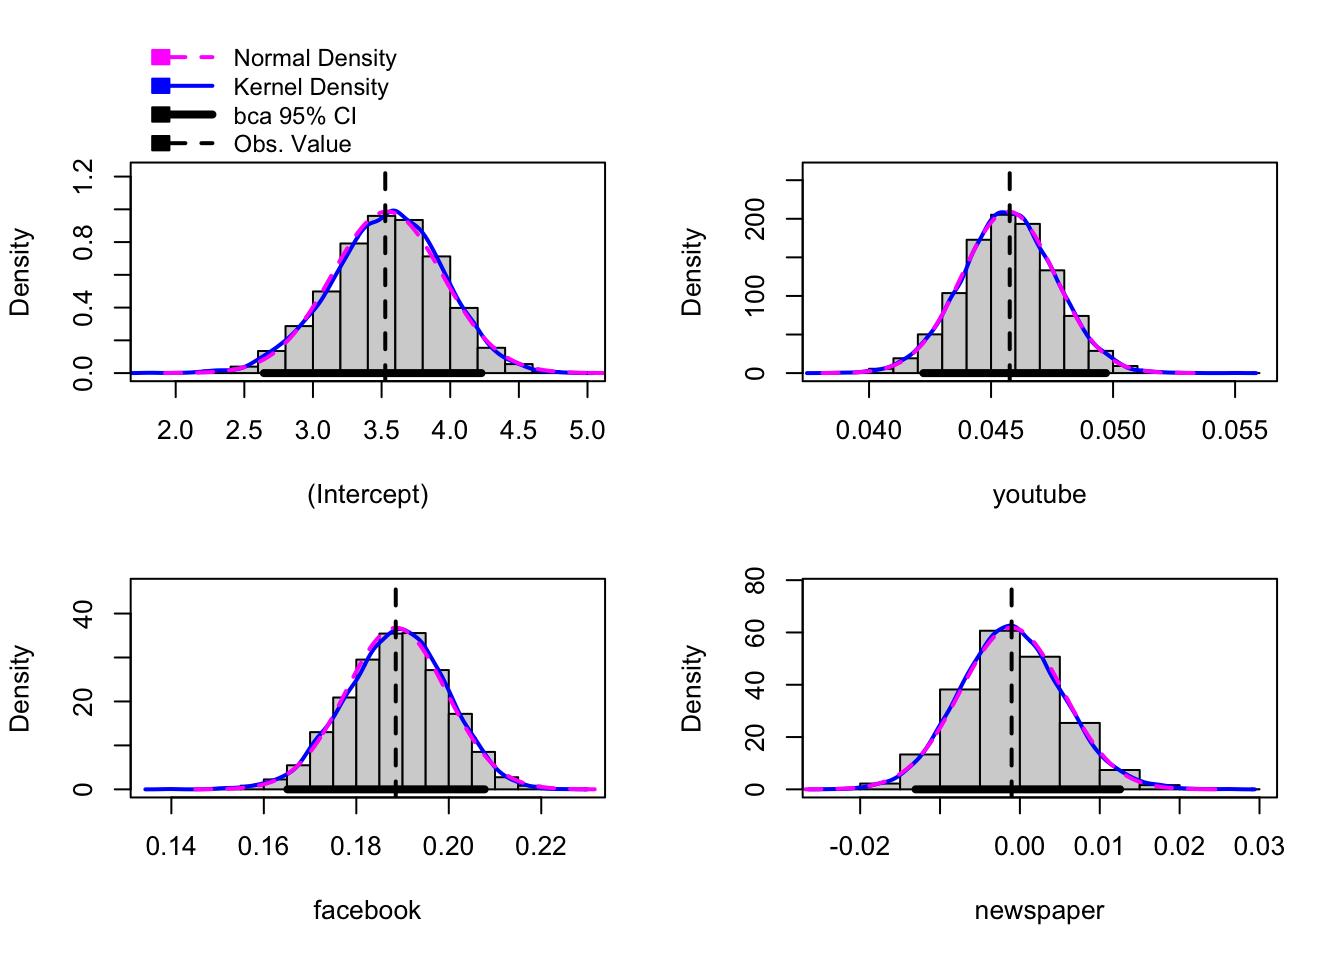
\includegraphics{applied_lecture_notes_files/figure-latex/unnamed-chunk-19-1.pdf}
Important to know how to interpret this. Even bootstrap CI aren't
necessarily precise. However, can check if our previous CI is
satisfactory by comparing with the bootstrap.

Question? the QQ-plot indicates normality not held. However the
resampling yields a beta estimate that is normal. One possible
explanation is CLT (large dataset).

\hypertarget{residual-resampling-parametric-boostrap}{%
\subsubsection{Residual resampling (parametric
boostrap)}\label{residual-resampling-parametric-boostrap}}

Suppose I fit a lm, i'm assuming the truth is a lm, and normality etc.
We can turn things around: i can generate data from my fitted data:
\(\tilde{Y}=X^T\hat{\beta}+\hat{\epsilon}\). We have two caveats, choice
for \(X\) and for \(\hat{\epsilon}\). For \(X\) we keep the design
matrix. We choose to resample \(\hat{\epsilon}\) along the residuals,
yielding \(\tilde{\epsilon}\)

\begin{Shaded}
\begin{Highlighting}[]
\NormalTok{boot.model2 }\OtherTok{\textless{}{-}}\FunctionTok{Boot}\NormalTok{(fit, }\AttributeTok{method=}\StringTok{"residual"}\NormalTok{, }\AttributeTok{R=}\DecValTok{1000}\NormalTok{)}
\FunctionTok{hist}\NormalTok{(boot.model2, }\AttributeTok{layout=}\FunctionTok{c}\NormalTok{(}\DecValTok{2}\NormalTok{,}\DecValTok{2}\NormalTok{))}
\end{Highlighting}
\end{Shaded}

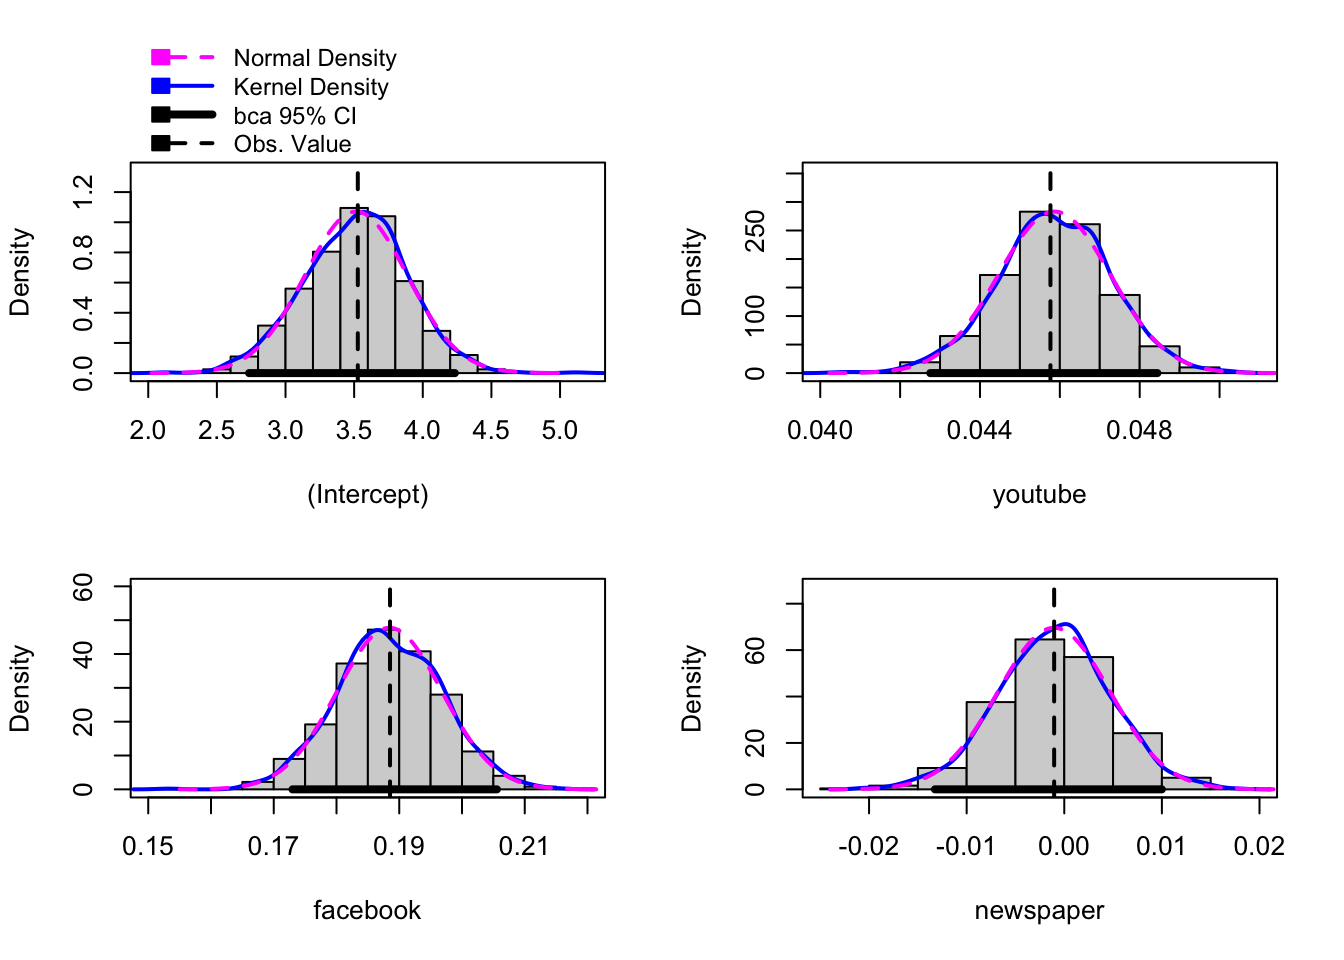
\includegraphics{applied_lecture_notes_files/figure-latex/unnamed-chunk-20-1.pdf}

\hypertarget{bootstrap-with-other-stats}{%
\subsubsection{Bootstrap with other
stats}\label{bootstrap-with-other-stats}}

\end{document}
